% !Mode:: "TeX:UTF-8"

\chapter{代码中间表示与质量评估度量提取}

%%%%%%%%%%%%%%%%%%%%%%%%%%%%%%%%%%%%%%%%%%%%%%%%%%%%%%%%%%%%%%%%%%%%%%%%%%%%%%%
\section{引言}

代码中间表示作为源代码和机器代码之间的抽象形式,能够在不丢失信息的前提下,准确地描述源代码的结构与行为。根据其表现形式的不同,代码中间表示可以大致分为三类\cite{2020MLIR}:第一类为线性中间表示,包括堆栈机代码、三地址码等;第二类为图中间表示,如抽象语法树、控制流图(Control Flow Graph,CFG)、数据流图(Data Flow Graph,DFG)以及调用图等;第三类则是线性中间表示与图中间表示的结合体。其中第二类基于图的中间表示能够有效地反映程序的控制流、数据流以及模块间的依赖关系,使开发者能够在分析过程中清晰地获取程序的执行逻辑、数据依赖关系及模块交互,从而为后续的代码优化、缺陷检测、重构等任务提供可靠的理论基础和技术支持。

在静态代码分析领域,尤其是针对代码质量评估的研究中,图中间表示已成为广泛应用的工具。例如,缺陷检测、代码复杂性分析、耦合度和内聚度的计算等研究方向,均依赖于图中间表示来描述程序的结构特征,并基于这些特征对代码质量提取相应的度量指标以进行定量评估。

针对代码质量评估的需求,已有大量研究从不同角度进行了探索,其中研究最为广泛的方向包括代码缺陷、内聚度、耦合性以及代码的复杂性等。为了帮助用户全面了解代码质量,本章基于抽象语法树,提取了方法调用链和全局变量使用链,进而生成了全局变量信息表和方法摘要表。基于这三个核心数据结构,进一步从四个关键维度提取代码度量指标,为后续的质量分析提供了全面的数据支持。



\section{基于clang的抽象语法树生成方法}
抽象语法树(Abstracted Syntax Tree,AST)是一种用来表现编程语言构造的树状结构,它把代码的语法结构以树形的方式进行了抽象化描述。在这个树形结构中,每一个节点都对应着代码中的某个元素,比如变量声明、语句或者是表达式等。从抽象语法树的根节点出发,代码逐步被拆解成更小的部分,直到最终到达叶节点,这些叶节点代表了代码中最基本的元素,如操作符或变量等。在抽象语法树中,节点之间的连接表明了它们之间的层级关系,即父节点与子节点的关系。通过这样的结构,AST 能够清晰地展示出代码的层次和结构,为编译器或其他工具分析和处理代码提供便利。


Clang 是由苹果公司发起的支持 C、C++、Objective-C 和 Objective-C++语言的编译器前端,负责对代码进行词法分析、语法分析和语义分析,对程序代码的分析和理解至关重要\cite{clang}。词法分析通过识别 Token 将程序代码分解成基本单元。语法分析在此基础上识别程序的语法结构,构造抽象语法树。语义分析消除语义模糊,生成属性信息,让计算机生成目标代码。而libclang 是 Clang 编译器的一个重要组成部分,它提供了一套用于解析源代码的程序接口。这些程序接口允许开发者在项目中使用 Clang 的强大语言解析和代码分析功能\cite{libclang}。本文使用libclang 生成AST ,提取代码中的调用和依赖关系,为后续进一步分析提供基础。


这里通过一个简单的例子来说明libclang的使用方式。如图 2-1 所示,这里定义了一个简单的 C 语言文件,文件中声明并定义了了两个方法和一个全局变量,主函数用于计算两个数的和。

\begin{figure}[h]
\centering
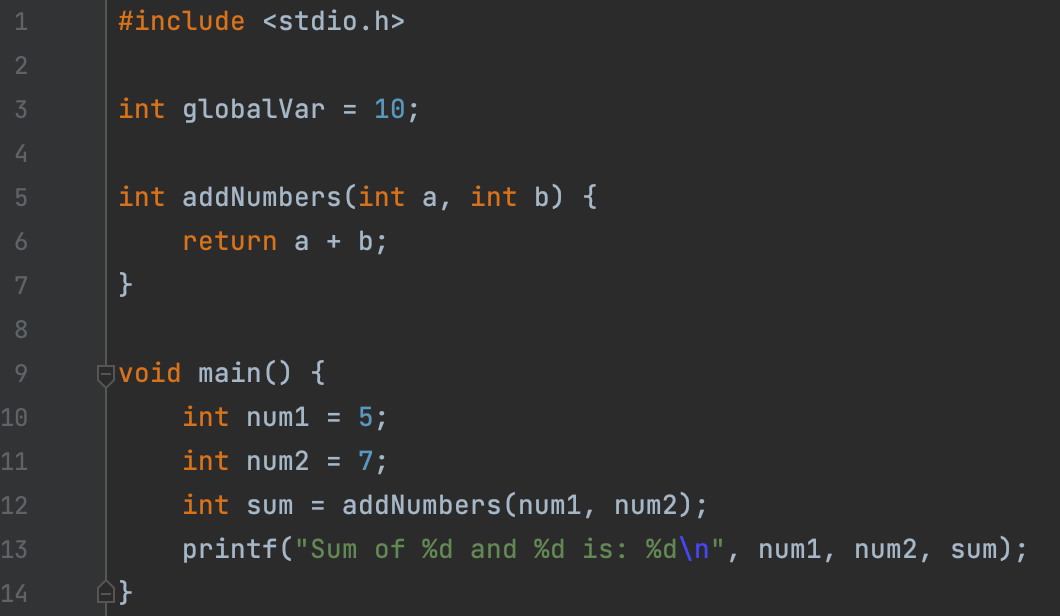
\includegraphics[width = 0.6\textwidth]{代码示例}
\caption{示例代码}
\end{figure}


这段代码由 Clang 解析生成抽象语法树后,得到的树结构如图 2-2 所示。

\begin{figure}[h]
\centering
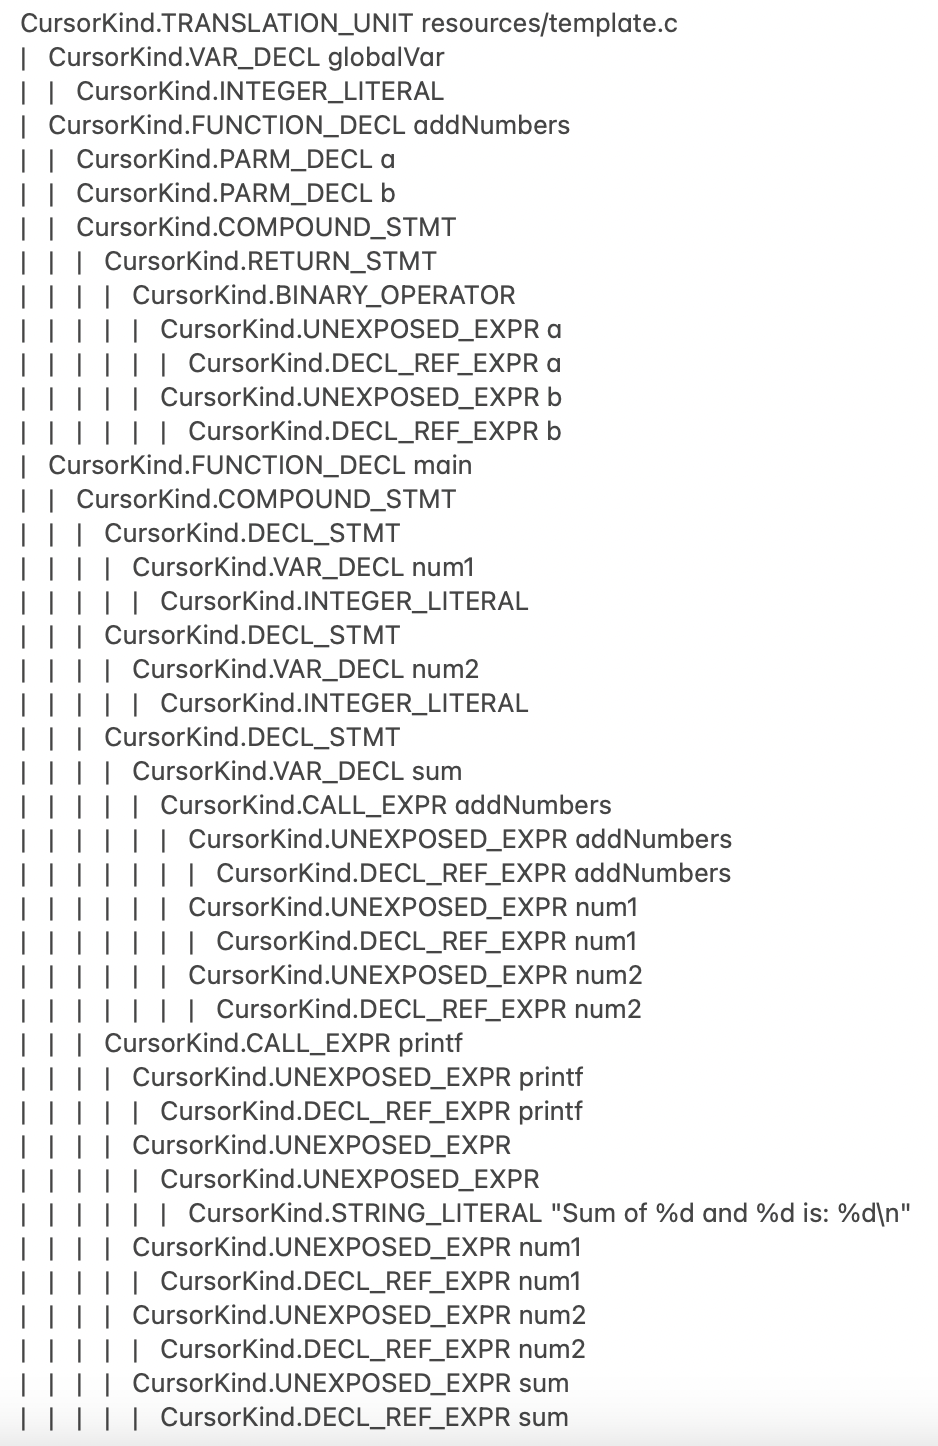
\includegraphics[width = 0.6\textwidth]{ast示例}
\caption{示例代码对应的抽象语法树结构}
\end{figure}

在 libclang 解析得到的抽象语法树中,游标(cursor)是一个核心概念,它作为一个指针或引用存在,每个 cursor 都与 AST 中的一个特定节点相对应,表示了源代码中的一个结构元素。通过操作 cursor,可以遍历整个 AST,访问和分析代码中的各种元素,如获取变量的类型、方法的参数列表、类的成员等。libclang 提供了一系列 API 函数来操作 cursor,例如:遍历 AST 中的 cursor、获取 cursor 的类型(如是否为方法定义、变量定义、变量引用等)、获取 cursor 所代表的源代码元素的名称、类型、位置等信息、获取 cursor 的父节点或子节点等。本文通过操作游标,遍历 AST,获取整个 AST的结构。


Clang 定义了一套节点类型标识。AST 的顶层节点类型是Translation\_Unit标签,表示一个翻译单元,对 AST 树的遍历,实际上就是遍历整个Translation\_Unit。Function\_Decl指的是方法定义,在 clang 中是不区分方法声明和方法定义的,统一用 Function\_Decl来标识,两个区分主要看是否有方法体,在 libclang 中提供了程序接口供开发者调用判断。Parm\_Decl 是参数节点,上面的例子中,方法 addNumbers 有两个参数 a 和 b。CompoundStmt 代表大括号,方法实现、struct、enum、for 的 body 等一般用此标签包起来。DeclStmt 是定义语句,里边可能有 VarDecl 等类型的定义,VarDecl 是对变量的定义。CallExpr 标签表示方法调用 Expr,子节点有调用的参数列表。ReturnStmt 表示返回语句。


\section{方法调用链提取与分析}
本文以整个代码项目为分析对象,代码中的方法为最小分析单元,方法之间的调用关系则是本文的分析基础。在使用 libclang 提取代码的抽象语法树后,遍历整棵树来提取方法之间的调用关系。这部分我们重点关注抽象语法树上的方法节点,以及方法节点内部的调用节点,分别对应着代码中方法的定义和方法内部对其他方法的调用。


对抽象语法树的遍历主要分为两次,第一次遍历的目的是获取所有的方法定义。首先提取所有的FUNCTION\_DECL 节点,它表示方法的定义,在该节点中可提取方法签名。在FUNCTION\_DECL 节点下,提取子节点 PARM\_DECL,该节点表示方法的参数列表,在该节点中可提取参数名称和参数类型等参数相关信息。然后提取FUNCTION\_DECL节点的子节点 VarDecl,该节点表示在该方法内定义的局部变量。在对方法进行分析时,我们本身不关心方法的内部实现,但是由于在 C/C++语言中,存在局部变量可以和全局变量重名的情况,在这里提取方法内定义的局部变量,方便后续在提取全局变量的使用时,排出同名局部变量的影响。除此之外,还需提取整个方法的 token 序列,所在文件以及作用域。


第二次遍历的目的是提取方法之间的调用关系。提取 FUNCTION\_DECL 节点
的子节点 CALL\_EXPR,该节点标签表示的是调用语句,可提取调用的方法名。注意,由于主要分析该项目中由开发者定义的方法之间的依赖关系,所以对于一些标准库方法的调用选择忽略,不进行提取。具体的提取流程如算法 2-1 所示。

分析结束后,将会获得每个方法的方法调用关系,对应于一个方法摘要表,包括项目
代码中所有的方法和方法之间的调用关系,除此之外还包括方法的参数表、方法主体和所在文件等其他信息。


\begin{algorithm}[H]
    \caption{方法调用链提取}
    \KwIn{项目中的所有代码文件: $files$}
    \KwOut{方法摘要表: $functions$}
    \KwLine
    \SetKwFunction{FMain}{scanAndAnalyze}
    \SetKwProg{Fn}{Function}{:}{}
    \Fn{\FMain{$files$}}{
        $functions \gets \{\}$ \KwComment{$\#$ 初始化方法摘要} \;
        \KwLine
        \KwComment{$\#$ 第一次扫描:收集方法的定义} \;
        \ForEach{$file \in files$}{
            $cursor \gets \text{libclang.parse}(file).cursor$ \KwComment{$\#$ 获取AST的根cursor} \;
            \texttt{traverse(cursor, 0, functions, file, True)} \KwComment{$\#$ 遍历AST,收集方法定义} \;
        }
        \KwLine
        \KwComment{$\#$ 第二次扫描:分析方法调用情况} \;
        \ForEach{$file \in files$}{
            $cursor \gets \text{libclang.parse}(file).cursor$ \KwComment{$\#$ 获取AST的根cursor} \;
            \texttt{traverse(cursor, 0, functions, file, False)} \KwComment{$\#$ 分析方法调用} \;
        }
        \KwLine
        \KwReturn{return $functions$} \;
    }
    \KwLine
    \SetKwFunction{FTraverse}{traverse}
    \SetKwProg{Fn}{Function}{:}{}
    \Fn{\FTraverse{$node, depth, functions, filePath, isFirstScan$}}{
        \If{$isFirstScan$}{
            \If{$node.kind == CursorKind.FUNCTION\_DECL$}{
                $function \gets \text{collectionInfo}(node)$ \KwComment{$\#$ C收集方法信息} \;
                $functions.\text{add}(function)$ \KwComment{$\#$ 将方法添加到方法摘要} \;
            }
        }
        \ElseIf{$node.kind == CursorKind.CALL\_EXPR$}{
            \texttt{parse(node)} \KwComment{$\#$ 分析被调用的方法} \;
        }
        \ForEach{$n \in node.get\_children()$}{
            \texttt{traverse(n, depth + 1, functions, filePath, isFirstScan)} \KwComment{$\#$ 递归遍历子节点} \;
        }
    }
    \end{algorithm}

\clearpage


\section{全局变量定义-使用链提取与分析}
在C/C++代码中,相同描述符修饰下的全局变量的定义、作用域、生命周期和方法是同级别的,所以在本文中,将全局变量也作为独立的代码单元进行分析。
全局变量定义-引用链的提取和方法的定义和调用提取类似,对 AST 的遍历主
要也分为两次。具体流程如图2-3。

\begin{figure}[h]
\centering
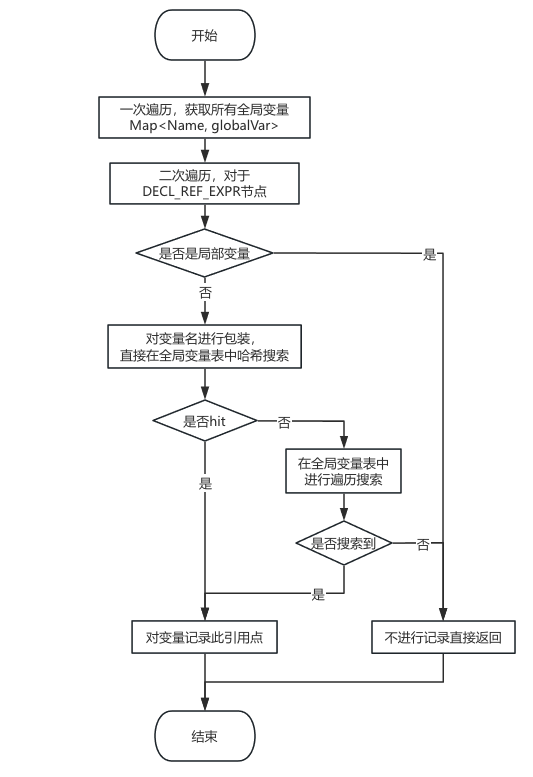
\includegraphics[width = 0.7\textwidth]{全局变量提取流程图.jpg}
\caption{全局变量提取流程图}
\end{figure}

第一次遍历获取所有的全局定义。首先提取所有的
VAR\_DECL 节点,它表示变量定义,然后提取节点中的变量名和变量类型。注
意,由于在 AST 中的节点标签中无法区分变量是否是全局的,所以这里根据节点在 AST
中的深度来判断是否是全局变量,并且在变量名前加上针对该项目文件的绝对路径,来
保证变量名的唯一性。在确定其为全局变量后,还需进一步提取该变量的作用域。在
C/C++语言中,static关键字可用于修饰变量和方法,意味着该变量或该方法只能在其所在文
件内使用,而不是全局可用,因此需要对其作用域进行判断。一次遍历提取到的结果是
一个全局变量表,这里使用哈希表 Map<Name, globalVar>的数据结构进行存储,方便对
全局变量进行查找。

第二次遍历的主要目的是提取全局变量的引用点。在方法节点子树中搜索
DECL\_REF\_EXPR 节点,该类型节点表示对变量的引用,这里首先判断被引用的变量是否是局部
变量,根据方法摘要表中该方法的相关信息可以判断,如果是则直接返回,因为我们不关心方法内的局部变量引用。如果不是,则证
明使用的是全局变量,首先在哈希表中进行查找该变量名,以节省检索时长,如果查找到了,说明
是在该文件中定义的全局变量,同时能够保证被 static 修饰的全局变
量的判断的准确性。如果没有查找到,则说明引用了别的文件中定义的全局方法,则在哈希
表中进行遍历查找,记录该全局变量被引用的方法。具体提取流程如图 2-3 所示。

分析结束后,则获得了每个全局变量的定义-引用链,对应于一个全局变量信息表,
包括项目代码中所有的全局变量和变量的引用点,除此之外还包括全局变量的类型、作
用域和所在文件等其他信息。

\section{基于代码中间表示的代码质量度量提取}

代码内聚度和代码耦合性是衡量软件设计质量的两个核心指标,它们直接反映了代
码模块化质量。代码内聚度指的是模块(如文件、类或组件)内部元素之间的相关性。高内聚度意味着模块内的所有元素都紧密地围绕着一个单一的、明确的功能,代码更容易理解和维护\cite{2014Service}。代码的耦合性则描述了模块之间的相互依赖。低耦合度意味着模块之间的依赖关系较小,每个模块都可以独立地执行其功能,而不需要过多地依赖其他模块。低耦合度的代码更容易测试和维护\cite{2013Ahe}。除此之外我们还考虑了代码的复杂性和代码缺陷,对


基于方法摘要和全局变量信息表,我们计算如下代码度量,用于分析代码质量。


\subsection{基于内聚度缺乏度的内聚性分析}

LCOM(Lack of Cohesion in Methods)系列指标是根据模块内聚度的缺乏程度来衡量模块的内聚度的指标。在本文中,
面向对象语言以类为研究范围进行计算内聚度,非面向对象的语言以文件为研究范围进行计算,类中的成员属性对应文件中的全局变量,类中的成员方法对应文件中定义的方法。LCOM 指标的核心思想是度量一个类中方法对实例变量(属性)的共享程度。不同版本的 LCOM 有着不同的计算方法和含义,体现了不同的侧重点。这里一共计算以下四个指标,

(1)LCOM1,含义是不引用相同字段的方法对数目\cite{1994Ametr}。计算公式如式(2-1)。
\begin{equation}
LCOM1 = C_{n}^{2}-e
\end{equation}

其中n 是文件中的方法总数,e 是引用相同字段的方法对。以图2-4为例介绍计算方式,其中椭圆表示方法,点表示变量,点在椭圆内表示该方法引用了该变量。LCOM1值为\(C_{6}^{2} - 5 = 10\)。

\begin{figure}[h]
\centering
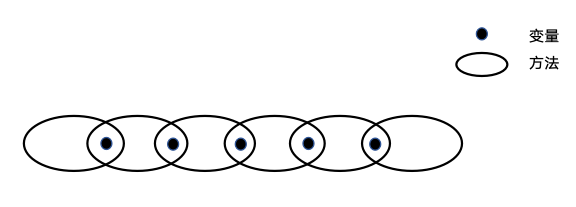
\includegraphics[width = 0.7\textwidth]{内聚度示例.jpg}
\caption{示例模块}
\end{figure}
    

(2)LCOM2,含义是不引用相同字段方法对与引用相同字段方法对数之差\cite{1996Coupling}。其计算公式如式(2-2)。

\begin{equation}
    {LCOM2}=\left\{
        \begin{array}
        {c}P-Q,  ifP\geq Q \\
        0,  otherwise
        \end{array}\right.
\end{equation}

其中,P 是不共享实例变量的方法对的数量,Q 是共享实例变量的方法对的数量。
如果 LCOM1 的结果为负数,则被置为 0。图2-4模块中,不共享变量的方法对P为10,共享变量的方法对Q为5,LCOM2值为P-Q=5。

(3)LCOM3是对前两种指标的进一步改进,其计算公式如式(2-3):
\begin{equation}
LCOM3 = \frac{\left( \frac{1}{a} \sum_{j=1}^a \mu(A_j) \right) - m}{1 - m}
\end{equation}

其中\( m\)为文件中的方法数,\( a\)表示文件中的变量数,\( mu(A_j)\)表示的是引用变量\(A_j\)的方法数。如图2-5所示的文件中有3个方法和3个变量,计算方式如图所示。
\begin{figure}[h]
\centering
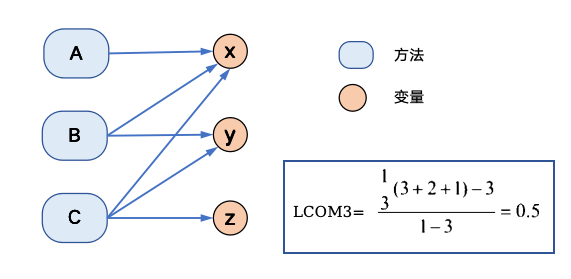
\includegraphics[width = 0.7\textwidth]{LCOM3.jpg}
\caption{LCOM3计算示例}
\end{figure}



(4)LCOM4,含义是以方法和变量为顶点,方法引用字段或方法之间有调用关系则两节点之间有条边构成图的连通分支数\cite{1995Measuring}。计算时,根据深度优先搜索的方式,计算图中的连通分支数,得到的值即为LCOM4。如图2-6所示的两个文件的LCOM4的值分别为2和1。

\begin{figure}[h]
\centering
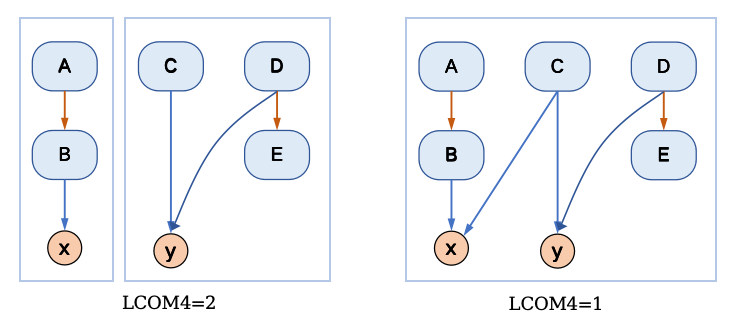
\includegraphics[width = 0.7\textwidth]{LCOM4.jpg}
\caption{LCOM4计算示例}
\end{figure}

\subsection{基于连通性的内聚性分析}
TCC(Tight Class Cohesion)和 LCC(Loose Class Cohesion)是用于衡量模块内
聚度的指标,这两个指标主要关注于模块中方法之间的连通关系,核心思想是通过
分析模块中方法如何相互作用以及如何访问共同资源(如全局变量)来评估模块的内聚度。


(1)TCC,含义是有连通关系的方法对数与总方法对数的比值\cite{1995Cohesion}。
TCC 关注于模块中方法之间的“直接连接”。如果两个方法直接共享访问同一个变
量,则认为这两个方法是直接连接的。计算公式如式(2-4)。
\begin{equation}
{TCC} = \frac{e}{C_{n}^{2}}
\end{equation}

其中\(n\)是文件中的方法总数,\(e\)是图中的直接连接边数。

(2)LCC则基于方法间接引用共同字段的关系进行计算\cite{1995Cohesion}。
LCC 除了考虑直接连接的方法对外,还包括了间接连接的方法对。如果两个方法不
是直接连接,但可以通过一系列的方法调用或变量引用来连接,则认为它们是间接连接的。LCC 的值基于模块中直接或间接连接的方法对占所有可能方法对的比例来计算。因此,LCC 的值通常不低于 TCC 的值,并且提供了一个更宽泛的模块内聚度视角。计算公式如式 (2-5):
\begin{equation}
{LCC=\frac{e+e_{indirect}}{C_{n}^{2}}}
\end{equation}

其中\(n\)是文件中的方法总数,\(e\)是图中的直接连接边,\(e_{indirect}\)是除直接连接边的边数。如图2-7是计算LCC和TCC的例子,左图中通过方法AB通过变量x直接连接,方法CD通过变量y直接连接,直接连接和间接连接都是2。而右图中直接连接是AB、BC、BC和CD,间接连接是AD和BD,因此计算结果如图。

\begin{figure}[h]
\centering
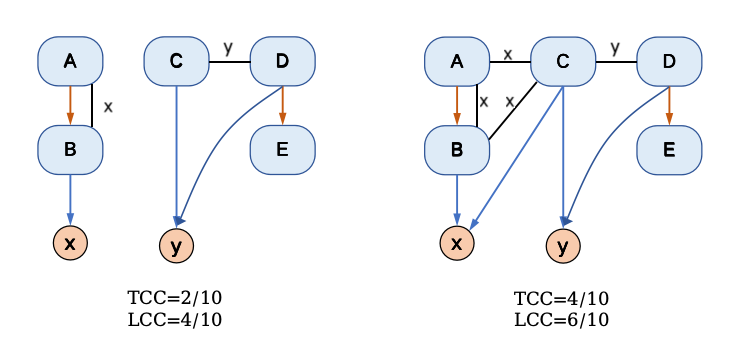
\includegraphics[width = 0.7\textwidth]{TCCLCC.jpg}
\caption{TCC和LCC计算示例}
\end{figure}


\subsection{方法间耦合性分析}

耦合是在软件架构中用来描述模块间相互依赖和连接程度的一个重要指标。耦合度的高低直接影响到系统的维护性和可扩展性。在现有的研究和实践中,耦合度通常被细分为六个等级,如表2-1所示,这些等级从高到低反映了模块间依赖的紧密程度。本文关注的是方法与方法之间的耦合性,方法间的耦合性反映了不同方法之间的依赖关系,它直接影响代码的可读性、可测试性以及后续的维护和扩展。通过深入分析方法级别的耦合性,研究方法如何通过参数传递、调用关系、共享全局变量等方式相互依赖,我们可以更准确地识别潜在的设计缺陷和优化机会,从而提高系统的模块化程度,增强系统的可维护性和可扩展性。

\begin{table}[htbp]
\caption{软件架构中耦合性分类}
\vspace{0.5em}\centering\wuhao
\begin{tabular}{ccccc}
\toprule
耦合性类别 & 描述 & 耦合程度 & 本文是否分析 \\
\midrule
内容耦合 & 模块直接访问或修改另一个模块的内部数据 & 6 & 否\\
公共耦合 & 模块访问同一公共数据环境 & 6 & 是 \\
外部耦合 & 模块共享全局简单数据结构 & 4 & 是 \\
控制耦合 & 模块传递控制信息,影响计算流程 & 3 & 否 \\
标记耦合 & 通过参数传递复杂数据结构信息 & 2 & 是 \\
数据耦合 & 通过参数传递简单数据 & 1 & 是 \\
\bottomrule
\end{tabular}
\end{table}


内容耦合是耦合度最高的一种形式,它表示一个模块能够直接访问或修改另一个模块的内部数据和结构。在方法级的耦合分析中,这种耦合形式通常不被考虑,因为方法间的直接数据访问往往通过参数传递或者 API 调用实现,而不是直接的内容访问。

公共耦合发生在多个模块共同访问某个全局数据环境时。这种数据环境可能是全局数据结构、全局变量或内存公共区域等。在提取到的全局变量表中,对于复杂数据结构如结构体和数组,其引用点所在的方法之间均存在公共耦合关系。


外部耦合与公共耦合相似,但区别在于它涉及的是对全局简单变量的访问。例如,当多个模块访问或修改相同的全局简单类型变量时,则这些模块之间存在外部耦合。


控制耦合指模块之间传递信息中包含用于控制模块内部的信息。在提取到的方法摘
要表中,遍历方法,如果该方法调用其他方法时,对应方法的参数列表中有变量决定了被调用方法中的计算流程,则方法之间存在控制耦合关系。由于本文不考虑分析方法内部的控制逻辑,因此不提取此种耦合。


标记耦合指通过参数表传递数据结构信息,调用时传递的是数据结构。在方法摘要
表中提取了方法的参数列表,包括参数名和参数类型,根据参数类型,可以确定
参数表中是否包含复杂类型。除此之外,在方法的调用表中,也提取了方法调用的
其他方法,结合这两个信息,即可确定两个方法是否存在着标记耦合关系。


数据耦合指通过参数表传递简单数据。与标记耦合类似,根据参数类型可以确定参
数是否全部为基本类型,结合方法调用表,即可确定两个方法是否存在数据耦合。
\subsection{方法扇入扇出度量分析}

方法的扇入(Fan-in)和扇出(Fan-out)是软件工程中用于衡量方法复杂性和模块
间依赖关系的两个指标。

\begin{figure}[h]
\centering
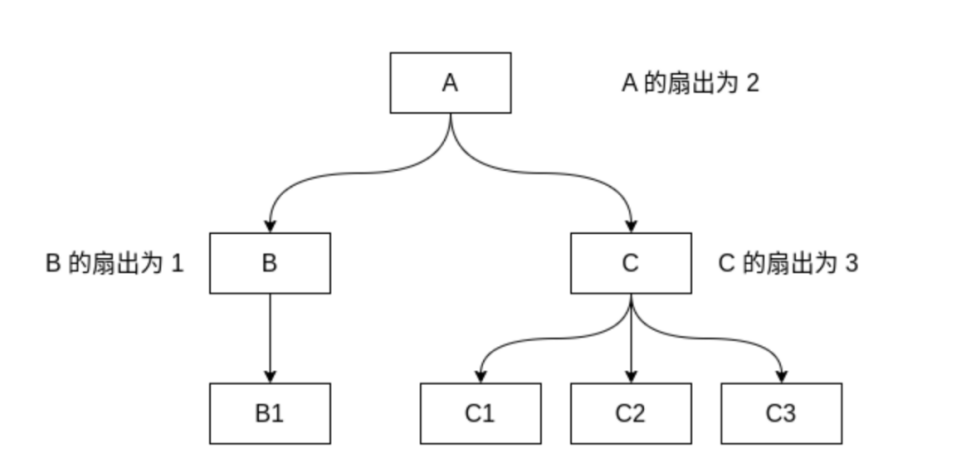
\includegraphics[width = 0.8\textwidth]{扇入扇出.png}
\caption{扇入扇出实例}
\end{figure}
    

扇入是指调用某个方法的不同方法的数量。它表示了一个方法对其他方法的依赖程
度。扇入值较高的方法通常被认为是重要的或核心的,因为它们被多个其他方法所依赖。
高扇入值可能意味着该方法执行了一个基础或共享的任务。


扇出是指某个方法直接调用的不同方法的数量。它表示了一个方法对其他方法的影
响程度。扇出值较高的方法可能更复杂,因为它们需要管理和协调更多的方法调用。高
扇出值可能意味着该方法具有较高的责任度,且可能更难以理解和维护。


本文中对于提取到的方法摘要表,遍历每一个方法,统计其调用方法的数量即可计算出该
方法的扇出值,再以该方法名在方法摘要表中搜索调用了该方法的方法,统计总数,得
到的值即为扇入值。

\subsection{基于静态检测工具的代码缺陷检测}

为了更准确地衡量代码质量,本文结合了静态代码分析工具 Cppcheck,对项目中的源代码进行检测和分析。Cppcheck 是一款开源的静态分析工具,专门用于检测 C/C++ 代码中的潜在错误和编码规范问题。它通过静态分析技术,扫描源代码,识别可能存在的内存泄漏、空指针解引用、未初始化变量等常见问题,并提供详细的诊断报告。与传统的编译器警告不同,Cppcheck 不依赖于程序的编译过程,它直接分析源代码的结构和逻辑,从而能够发现更广泛的潜在问题,尤其是那些难以通过常规测试手段捕捉到的错误。

在本研究中,Cppcheck 的检测结果被视为代码质量评估的重要组成部分。Cppcheck会根据问题的严重性和类别将检测出的问题如表2-2所示的六类。

\begin{table}[htbp]
\caption{cppcheck报告问题分类}
\vspace{0.5em}\centering\wuhao
\begin{tabular}{cccc}
\toprule
类别 & 描述 \\
\midrule
error &  严重错误 \\
warning & 潜在的错误或不推荐的做法 \\
style & 代码风格问题,通常与代码格式、命名约定等相关 \\
performance & 性能问题,表明当前方式可能效率不高 \\ 
portability & 平台相关问题,可能导致在不同环境出现不同行为 \\
information & 额外的信息或建议 \\ 
\bottomrule
\end{tabular}
\end{table}

检测结果中包括了诸如错误、警告和代码风格问题等不同级别的信息,这些信息帮助开发者识别代码中的潜在问题并及时修复,进而提高代码的可维护性和健壮性。

Cppcheck 提供的报告与其他度量指标相结合,共同构成了全面的质量评估体系。用户可以根据检测报告对代码质量进行更细致的判断和分析,从而为后续的优化和重构提供科学依据。通过这种方式,本研究实现了对代码质量的多维度综合评价,为开发者提供了更为精确的质量检测和改进方向。


\section{实验结果与分析}

\subsection{实验数据与评价方式}

1. 实验数据

本文从影响力或社区活跃程度的角度出发,收集了表2-2中所示的软件项目为示例项目进行实验。这些项目在github上的收藏数均在千以上,说明这些项目在开源社区中有着一定的影响力,使用范围比较广泛。除此之外,这些项目有着比较活跃的社区,说明其还在不断更新迭代过程中,所以能提供较为丰富的变更历史,以供后续的实验分析。

\begin{table}[htbp]
\caption{示例项目}
\vspace{0.5em}\centering\wuhao
\begin{tabular}{cp{6cm}ccc}
\toprule
项目名称 & 项目简介 & 代码行数& 提交数 & 收藏数 \\
\midrule
TheAlgorithms & 各种算法的开源实现,涵盖了计算机科学、数学和统计学等领域 & 24645 & 1536 & 57k \\
antiword-0.37 & 提取 Microsoft Word 文档内容的工具 & 34725& - & 13k\\
jemalloc-5.3.0 & 通用的malloc(3)实现,强调碎片避免和可扩展的并发支
持  &83525& 3530 & 9k \\
libbpf-1.1 & linux 内核观测技术的一个脚手架库 & 127927 & 2375 & 1.9k \\
librdkafka-2.1.0& Apache Kafka 的 C/C++ 客户端库 & 154951 & 4430 & 18k \\
FFmpegKit-5.1.0 & FFmpeg 工具包 & 450998 & 369 & 3.7k \\

\bottomrule
\end{tabular}
\end{table}

2. 实验过程和评价方式

将实验项目的github仓库克隆到本地,对每个项目进行按前文所述步骤提取代码中间表示,包括抽象语法树、方法摘要表和全局变量信息表,再进一步按2.5节所述方法,提取代码质量度量和缺陷信息。在提取到质量度量后,筛选质量较差的代码分析结果报告给用户,收集用户的反馈,衡量方法的有效性。报告的标准如下:

(1)内聚度

内聚度是衡量一个模块内部各个组件(本文中是方法和全局变量)之间关系的紧密程度的指标。内聚度越高,则意味着模块内的各个部分越紧密,职责明确且功能聚焦。然而,仅凭数值的计算,用户可能难以直观理解模块的内聚度高低。因此本文通过对同一项目中各模块内聚度进行排名,向用户报告内聚度最差的前5\%模块,以帮助用户识别和定位项目中内聚度较差的模块。随着用户不断进行改进,模块的内聚度将逐步提升并收敛,最终整个项目达到平衡的状态。

(2)耦合性

本文中提取了四种不同的耦合类别,每种类别的耦合程度并不相同,数据耦合、标记耦合、外部耦合、公共耦合,耦合程度依次递增。\inlinecite{迟曲2011关于软件设计的模块独立性分析}中提到数据耦合是最佳的耦合类型,而外部耦合和公共耦合则对系统的质量和维护性有负面影响。这是由于数据耦合和标记耦合都通过参数传递数据,方法的输入输出明确,易于测试和维护,而外部耦合和公共耦合共享公共数据,可能会影响程序的可测试性和问题的排查诊断。

本文进一步将代码是否处于同一模块考虑在内,因为对于同一模块内,代码往往有共同的上下文和职责范围,因此可适当对耦合标准放宽。因此对与在同一模块内的方法,报告公共耦合,对于不在同一模块内的方法,报告外部耦合和公共耦合,将这两种情况作为不良耦合报告给用户。

(3)扇入扇出

传统标准中要求尽量高扇入低扇出,高扇入表示其他模块依赖该模块,模块的功能可能是系统中其他模块的核心或基础,复用性较好;低扇出表示该模块没有过多地依赖其他模块,因此它具有更高的独立性,更易维护。同内聚度类似,仅计算数值或统一设置阈值的方式,用户难以直观理解,因此这里也对同一项目中扇入扇出值进行排序,向用户报告最差的前5\%的方法。

(4)静态分析工具

本文结合了静态分析工具Cppcheck对项目代码进行检测。考虑到Cppcheck的严重等级分类能从错误、警告、风格、性能、未定义行为等多个角度提供细致分析,每个类别都关注特定的代码问题,不仅帮助开发者准确识别出可能导致崩溃或异常行为的缺陷,还能够进行规范检查,发现影响程序效率、可读性、资源管理等方面的潜在问题。因此本文将向用户报告表2-2中六种类型的问题,作为质量评估的一部分,提供给用户进行判别。

总的来讲,这四种度量向用户报告的标准如表2-4所示。

\begin{table}[htbp]
\caption{各度量报告标准}
\vspace{0.5em}\centering\wuhao
\begin{tabular}{cccc}
\toprule
度量 & 报告标准 \\
\midrule
内聚度 &  6项指标分别报告内聚度最差的前5\%模块 \\
\multirow{2}{*}{耦合性} &  同模块内报告公共耦合\\
                        & 不同模块报告公共耦合、外部耦合 \\
扇入扇出 & 分别报告最差的前5\%方法 \\
静态工具检测 &  报告6种类型问题\\ 
\bottomrule
\end{tabular}
\end{table}

为了验证质量度量的可靠性与实用性,本文邀请了四位经验丰富的软件开发者,对报告的每一项的准确性和可接受性进行评估。评估的标准包括以下几个方面:

\begin{itemize}
    \item 内聚度差、耦合不良、扇入过低、扇出过高和缺陷的检测结果是否能为用户所接受:评估这些指标的报告内容是否准确反映了代码中的问题,且是否能够为开发者提供有效的指导。
    \item 指标的解释与建议是否有助于代码优化:不仅是检测结果本身,还需要评估报告中对检测结果的解释是否充分。
    \item 报告结果与实际代码质量的关联性:通过比较报告中的分析结果与开发者实际编码过程中所遇到的问题,验证报告的实用性。
\end{itemize}

对于报告的每一项,如果用户认为符合标准,则认为用户接受对应的结果,则将对应的项反馈结果标记为1,统计用户的接受率,接受率指标计算公式如式(2-6)
\begin{equation}
    AR_n =  \frac{\frac{1}{N} \sum_{i=1}^{N} A_i}{T} \times 100\%
    \end{equation}
其中AR表示接受率,A表示开发者接受的项数,T表示报告的总项数,N表示软件开发者数。

\subsection{实验结果与实例分析}
1. 内聚度实验结果及实例分析

(1)内聚度实验结果

表2-5展示了对于内聚度报告项用户的接受率,从实验结果可以看出,该方法表现良好,可靠性较高。具体来讲,指标基本都在70\%以上。通过进一步对比,发现在TheAlgorithms、antiword等比较简单的项目中,内聚度在6项指标中常出现相同的接受率,经过分析发现这是因为在同一项目中,尽管6项指标的计算方式和侧重点都不同,但是最差的前5\%基本上是重合的,这意味着一个模块如果在LCOM1中表现的很差,在其他指标中也通常表现得很差,这符合通常认知,同时也侧面验证了指标的准确性。但是对于FFmpegKit等较复杂的项目,6项指标则不太相同,体现了不同内聚度计算方式的侧重点。

\begin{table}[htbp]
\caption{内聚度接受率}
\vspace{0.5em}\centering\wuhao
\begin{tabular}{ccccccc}
\toprule
项目名称 & LCOM1 & LCOM2 & LCOM3 & LCOM4 & TCC & LCC \\
\midrule
TheAlgorithms & 89.2 & 74.9 & 74.9 & 89.2 & 74.9 & 74.9 \\
antiword-0.37  & 91.3 & 84.2 & 84.2 & 91.3 & 84.2 & 84.2 \\
jemalloc-5.3.0 & 82.2 & 82.2 & 82.2 & 82.2 & 88.6 & 88.6 \\
libbpf-1.1 & 87.3 & 83.4 & 87.3 & 87.3 & 93.7 &  93.7 \\
librdkafka-2.1.0 & 73.7 & 73.7 & 73.7 & 73.7 & 78.4 & 78.4 \\
FFmpegKit-5.1.0 & 71.3 & 69.2 & 74.9 & 76.6 & 89.3 & 84.9 \\

\bottomrule
\end{tabular}
\end{table}


(2) 内聚度实例分析

对内聚度实验结果进行进一步分析,这里选取 antiword 项目中的内聚度表现最差的模块 misc.c 文件模块进行分析。为了更好地理解这一现象,进一步检查了该模块的源代码,并对其结构进行了统计分析。具体来看,misc.c 文件中一共定义了 1 个全局变量和 15 个方法,其中 11 个方法并未被同一模块内的其他方法调用,只有 3 个方法之间存在相互调用关系,而仅有 2 个方法使用了该模块定义的全局变量。

通过这个结果可以发现,尽管该模块包含了一定数量的方法和变量,但模块内各个方法和变量之间的依赖关系极为薄弱。大部分方法相互之间没有调用关系,且仅有少数方法与全局变量发生交互。这样的结构表明,模块内的功能划分较为松散,各个功能单元之间缺乏必要的协作和紧密联系。因此,该模块的内聚度较差,功能的集中性和一致性较低,导致其内聚度值显著较低。因此,通过对 misc.c 文件内聚度的分析,我们不仅可以得出该模块的内聚度较差的结论,还能为未来的重构和优化提供指导意见。例如,增强模块内部方法之间的调用关系,优化变量的使用方式,以提高模块的内聚度,从而提升系统的整体质量和可维护性。

2. 其他度量实验结果及实例分析

表2-6展示了对于其他度量报告项用户的接受率,从实验结果可以看出,不同项目在各项度量指标上的接受率存在一定差异。大部分项目的耦合性接受率较高,而扇入扇出的接受率普遍较低,大部分的项目上只达到了40-50\%的水平,而所有项目对静态工具检测出来的缺陷上的接受率都较高,说明静态工具的可靠性较好。接下来对所有指标的实验结果进行进一步分析。

\begin{table}[htbp]
\caption{其他度量接受率实验结果}
\vspace{0.5em}\centering\wuhao
\begin{tabular}{cccc}
\toprule
项目名称 & 耦合性接受率 & 扇入扇出接受率 & 静态工具缺陷接受率 \\
\midrule
TheAlgorithms & 99.2 & 87.6 & 100.0 \\
antiword-0.37 & 84.2 & 56.4 & 98.0 \\
jemalloc-5.3.0 & 77.8 & 66.3 & 100.0 \\
libbpf-1.1 & 68.3 & 42.1 & 100.0 \\
librdkafka-2.1.0 & 63.7 & 48.7 & 98.8 \\
FFmpegKit-5.1.0 & 54.0 & 43.3 & 94.6 \\
\bottomrule
\end{tabular}
\end{table}

(1)耦合性结果分析和实例分析

耦合性的接受率在几个项目中的表现不尽相同。对于结构较为简单的项目,如antiword和jemalloc,接受率均能达到较高的水平,在TheAlgorithms项目上甚至能达到99\%以上的接受率。而对于更大型更复杂的项目,接受率则略微降低。

进一步分析如此表现的原因,对于TheAlgorithms,这个项目是对各种算法的开源实现,模块和模块之间几乎不存在相互依赖和调用的情况,每种算法独立开发,实际上是库函数,仅在需要时供开发者调用。总的来讲,简单项目结构较为简单,各个模块功能明确,职责聚焦,所以耦合性不良的样例很少,共检测出15例。维护起来也更加容易,用户更容易接受。

而在复杂项目中,如FFmpegKit,耦合性接受率相较其他项目低一些。这里以FFmpegKit项目中不被用户所接受的样例进行分析。在这个样例中,方法probe\_file与另外三个模块的方法发生了公共耦合,具体来讲这几个方法共同使用了fftools\_ffprobe.c文件中定义的全局变量nb\_streams,这是一个整数。而不被用户所接受的理由是,这个全局变量实际上是一个共享全局状态,它代表了流的数量,需要在不同平台上保持一致,如表中所示,需要在android、linux、apple的环境中都保持一致,才能保证程序的正确性和一致性。在这种情况下,多个方法访问并操作该全局变量是合理的,因为这种做法确保了平台间的一致性。

\begin{table}[htbp]
\caption{FFmpegKit项目中不被用户接受的不良耦合实例}
\vspace{0.5em}\centering\wuhao
\begin{tabular}{cp{12cm}}
\toprule
共同访问变量 & 方法名 \\
\midrule
\multirow{4}{*}{nb\_streams} & ffmpeg-kit/apple/src/fftools\_ffprobe.c@probe\_file \\
                              & ffmpeg-kit/android/ffmpeg-kit-android-lib/cpp/fftools\_thread\_queue.c@tq\_alloc  \\
                              & ffmpeg-kit/linux/src/fftools\_thread\_queue.c@tq\_alloc  \\
                              & ffmpeg-kit/apple/src/fftools\_thread\_queue.c@tq\_alloc  \\
\bottomrule
\end{tabular}
\end{table}

通过对这个样例的分析可以看出,对与大型、复杂的软件项目来讲,各模块和方法之间的依赖关系可能已经非常复杂,需要大量时间来理解现有结构并分析方法间的相互影响,对于某些功能,也的确缺乏耦合性更低的实现方式,所以接受率更低。

(2)扇入扇出接受率分析

对于扇入和扇出值指标,观察到该指标的接受率较低。通过实例分析发现,大多数项目的开发模式并不完全符合高扇入、低扇出的设计原则。

特别是在低扇入的报告项中,接受率尤为偏低。实际分析表明,许多方法仅被单次调用,虽然这些方法的复用性较差,但它们更为独立,且较少依赖于其他模块的实现。这种独立性使得这些方法更容易进行单独测试、维护和扩展。考虑到软件的长期发展,这些低扇入的方法未来仍有可能被其他模块调用。因此,低扇入方法在某些情况下是有其优势的,用户难以直接接受此类报告项,因此拉低了整体的接受率。

而对于高扇出的报告项,大部分是可以接受的,但是也存在某些高扇出的方法是合理的,比如有些高扇出方法实际上是中心化的模块。

\begin{figure}[h]
\centering
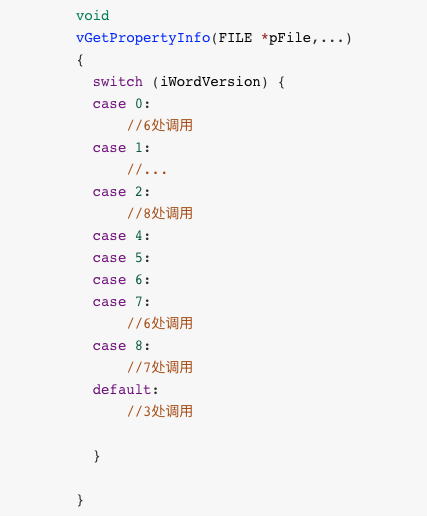
\includegraphics[width = 0.5\textwidth]{扇出高例子.jpg}
\caption{vGetPropertyInfo方法结构}
\end{figure}
    

这里以antiword项目中properties.c文件的vGetPropertyInfo方法为例,该方法主要根据传入的Word版本,从文档中提取各种属性信息。该方法的扇出度为30,是项目中扇出度较大的一个,方法可能复杂度过高,因此被报告属于不良的扇出,但这一报告并未得到用户的接受。其原因在于,该方法的核心结构是一个包含多达9种不同情况的 switch 语句,每种情况又细分为多个子情况,因此导致总共产生了30个方法调用。该方法的合理性在于通过清单式方式集中处理所有功能逻辑,使得用户能够一目了然。此设计不仅减少了冗余代码,避免了方法调用链过长带来的可读性问题,还降低了因方法调用所带来的额外开销,从而优化了整体系统的效率。因此,尽管该方法具有较高的扇出度,其设计思路仍然是有效的,符合高效代码的要求。

(3)静态工具检测接受率分析

静态工具检验得到的代码缺陷的接受率是最高的,经过分析发现只有个别错误,如平台相关问题,与特定编译器相关的警告等不容易被开发者所接受,因为这并不是代码本身的质量问题。


经过分析可以发现,这些度量指标有一定的有效性,但是这些度量聚焦的往往是范围较小的质量问题。如模块内、方法内甚至语句级的质量问题。面对更大规模的软件代码时,无法反映其在架构上的缺陷,难以帮助开发者从宏观的角度上指导代码维护。

\section{本章小结}

本章实现了对代码中间表示的提取及质量评估度量的计算。首先,本文基于 libclang 工具对软件项目进行抽象语法树提取,并在此基础上进一步构建了方法摘要表和全局变量信息表。随后,基于提取得到的中间表示,分别介绍了基于内聚度缺乏度和基于连通性的内聚度分析,介绍了方法间耦合性分析以及扇入扇出的提取和分析,通过这几种分析手段提取了 8 个代码质量指标和 6 种耦合关系。本章通过一系列实验验证了度量指标的有效性,但是发现其只能聚焦于范围较小的质量问题,无法反映软件系统在架构上的缺陷,难以帮助开发者从软件代码的宏观角度上指导软件维护。

%%%%%%%%%%%%%%%%%%%%%%%%%%%%%%%%%%%%%%%%%%%%%%%%%%%%%%%%%%%%%%%%%%%%%%%%%%%%%%%
\chapter{面向代码质量评估的变更影响分析方法研究}
\section{引言}

软件变更是软件维护的核心环节。对软件系统的修改可能引发系统其他部分的不良副作用或连锁反应。而变更影响分析的目标在于识别变更的涟漪效应,它能够破除模块和模块之间的界限,从宏观角度上分析代码之间的相互影响,帮助开发者安全地进行变更。本文的研究对象是C/C++项目,研究粒度设定为方法级别。方法之间的变更影响可以分为以下三种类型:

(1)直接调用关系:这种变更影响关系是最直接的。例如,若方法 funcA 调用了方法 funcB,那么当 funcB发生变化时,所有调用 funcB 的方法,包括funcA都会受到该变更的影响,最显然的,如果funcB的签名发生更改,funcA必须随之修改,否则将调用失败,甚至编译错误。

(2)共同调用关系:当方法 funcA 和 funcC 同时调用方法 funcB 时,funcA 与 funcC 之间会形成变更影响关系。这种关系实际上是第一种类型的扩展,通常情况下,funcB 的变化会引起 funcA 和 funcC 的同步修改。

(3)逻辑上存在变更影响关系:在这种类型的变更影响关系中,尽管方法之间没有直接调用关系,也不共同调用某个方法,但它们的实现逻辑或所操作的数据之间存在某种隐含的关联。具体来说,这种关系可能源于它们共同维护某个数据的一致性、共享某些资源,或其功能逻辑有某种预期联系。因此,当某个方法发生变化时,可能会间接影响到其他方法的行为或结果。

其中前两种类型可在代码的静态结构中直接显现,通过传统静态分析方法甚至开发工具即可捕捉,第三种则属于逻辑型变更影响,只能通过开发者人工进行分析提取,而正是因为此种关系的存在,导致了开发者难以理解软件架构、难以安全变更的问题出现。因此为了解决此痛点,本文实现了基于依赖关系闭包的传统分析方法,并提出了三种新的变更影响分析方法,从而能够全面挖掘这三种类型的变更影响关系,并且通过深入分析挖掘到的变更影响关系,对每一类影响分析其带来的质量问题和提出优化方向。

\section{基于依赖关系闭包的变更影响分析}

变更影响分析的主要目标是识别软件系统中由代码修改引发的涟漪效应,从而有效防止变更产生的副作用。这一过程旨在帮助开发者全面评估变更可能带来的直接和间接影响,并制定相应的测试与维护策略。在代码变更影响关系分析中,依赖关系传递闭包分析被广泛应用,这是一种基于静态依赖关系的技术手段,通过识别代码模块间的关联性,精准划定受变更影响的范围\cite{2021Improving}。其核心思想是利用依赖关系的传递性,通过构建和分析依赖图,揭示所有可能受到影响的代码模块或单元。

依赖关系传递闭包分析的基本假设是,软件系统中的各个代码单元(如方法或全局变量)存在不同程度的直接或间接依赖。通过对这些依赖关系的深入分析,可以识别代码变更对系统其他部分的潜在影响。本文以方法和全局变量为基本分析单元进行变更影响分析。

(1)代码预处理

在进行代码变更影响分析之前,首先需要将源代码转化为一种可供进一步分析的程序模型。该模型通常由一组能够描述代码结构和依赖关系的数据结构组成,其目的是通过抽象化和结构化的方式,将复杂的代码逻辑转化为更易于分析的形式。本文对代码进行预处理,核心思想是以抽象语法树、全局变量信息表和方法摘要表为基础,构建程序的系统依赖图,为后续的依赖关系分析和影响范围评估提供数据支撑。

首先,使用libclang对源代码解析生成抽象语法树。在生成抽象语法树之后,进一步构建全局变量信息表和方法摘要表。全局变量信息表用于记录程序中所有全局变量的相关信息,包括变量名、定义位置,以及使用了该变量的方法的名称。通过这些信息,能够明确全局变量与方法之间的依赖关系,从而识别代码中跨模块或跨方法的依赖。方法摘要表旨在对程序中的方法进行全面的结构化描述。该表包含每个方法的签名信息(如方法名和参数列表)、定义位置(如所在文件)、方法内定义的局部变量,以及方法调用的其他方法列表。这些信息不仅可以用于分析方法间的调用关系,还可以帮助区分局部变量和全局变量,从而更精确地提取依赖关系。

这些数据结构共同构成分析所需的程序模型,为依赖关系的提取和后续的传递闭包计算提供基础支持。

(2)构建依赖关系图

依赖关系图的构建依赖于前述提取的全局变量信息表和方法摘要表。在构建过程中,首先需要识别代码中的直接依赖关系,包括方法调用和变量引用等。前面提取的全局变量信息表和方法摘要表已经包含了这些直接依赖关系的信息。接下来,依赖关系被形式化为一个有向图,图中的节点代表代码中的基本元素,本文中是方法和全局变量,而有向边则表示这些元素之间的依赖关系。如果方法A调用了方法B,那么在依赖关系图中增加一条从节点A指向节点B的有向边。如果方法A引用的全局变量C,那么在依赖关系图中增加一条从节点A指向节点C的有向边。通过这种方式,依赖关系图不仅能够系统地表示代码中各个元素之间的直接依赖关系,还能为后续的变更影响分析提供结构化的图形模型。

(3)执行变更影响分析

接下来,基于依赖关系图进行变更影响分析,实际上是对方法之间变更影响关系的全面识别与提取过程。具体而言,这一过程旨在确定哪些方法在代码变更时可能受到影响,以及这些影响的传播路径。本文基于方法和方法之间的以下两种关系RBM(relationships between methods)来识别受影响的方法集IMS(impacted method set),如式(3-1)所示。
\begin{equation}
\begin{array}{l}
R B M=C A L L \cup R E T U R N \text { where } \\
(f, g) \in C A L L \Longleftrightarrow f(\text { transitively)calls } g, \\
(f, g) \in R E T U R N \Longleftrightarrow f(\text { transitively)returns into } g
\end{array}
\end{equation}

这里以方法f和方法g的关系为例,CALL方法和RETURN分别代表f和g的调用和被调用关系。

对于依赖关系图中的每个节点,我们需要计算该节点的传递闭包。传递闭包是指从某个特定节点出发,根据上文定义的依赖关系和图的可达性,可以直接或间接到达的所有节点的集合。换言之,传递闭包反映了节点之间的依赖链条以及影响传播的范围。为了高效地计算传递闭包,利用广度优先搜索遍历图中的各个节点及其依赖边,进而识别出所有直接或间接依赖于某个节点的其他节点。每次从某个节点出发时,都会跟踪并记录通过依赖关系可到达的所有节点,最终形成该节点的完整传递闭包。传递闭包的具体计算公式如式3-2

\begin{equation}
\begin{array}{l}
I M S^{(N)}=I M S_{C A L L}^{(N)} \cup I M S_{R E T U R N}^{(N)} \\
I M S_{ {RETURN }}^{(N+1)}=\bigcup_{{define } \in \left(I M S_{R E T U R N}^{(N)}}-I M S_{R E T U R N}^{(N-1)}\right)} I M S({ define }) \\
I M S_{C A L L}^{(N+1)}=\bigcup_{ {define } \in\left(I M S_{C A L L}^{(N)}\right)} I M S( { define }){, define } \in \\
\left(I M S_{C A L L}^{(N)}-I M S_{C A L L}^{(N-1)}\right) 
\end{array}
\end{equation}

在变更影响分析的具体应用中,我们假设依赖图中的某个方法节点发生了变更,并按上述公式进行计算,最终得到的节点集合中,所有的节点(即方法)都与初始变更的节点存在某种直接或间接的依赖关系。这些方法可以视为受变更影响的范围,意味着它们在该方法变更后,可能会因为依赖关系的传递而受到影响。通过这一分析,我们不仅可以识别出受影响的直接方法,还能揭示出那些通过多次间接依赖而受到影响的方法,帮助开发者全面了解变更的潜在影响范围。


以图 3-1 为例,在这个例子中,一共有6个方法,其中方法 funcA 调用了 funcB 和funcD,funcB 调用了 funcC。在对 funcB 进行变更影响分析时,会直接影响到 funcA和funcC,根据依赖关系闭包,会间接影响到funcD。所以与 funcB 有变更影响关系的方法集合为\{funcA, funcC, funcD\} 。

\begin{figure}[h]
\centering
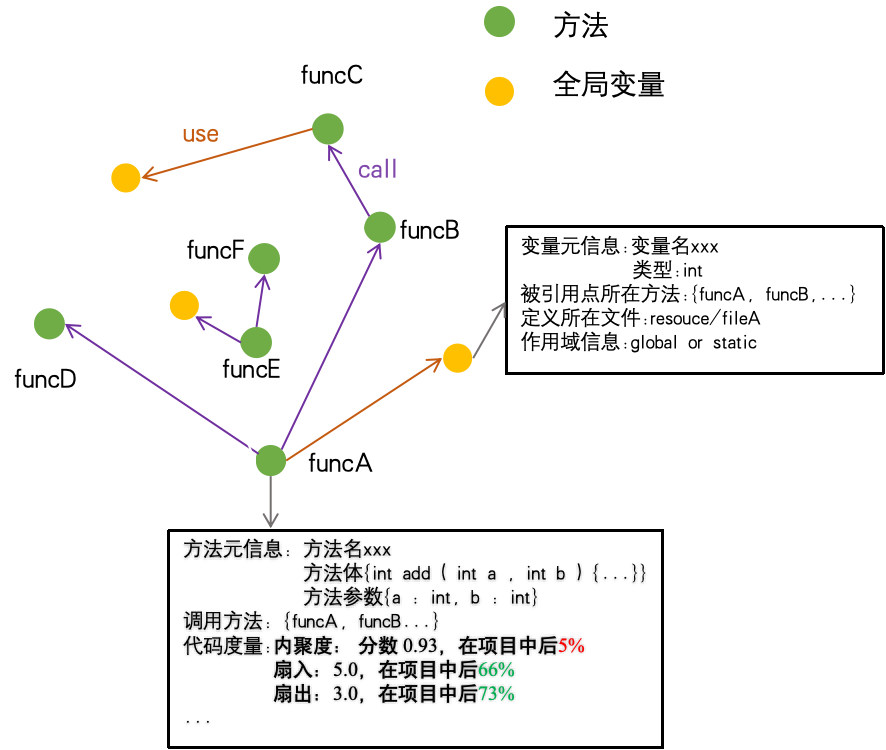
\includegraphics[width = 0.6\textwidth]{依赖关系示例.png}
\caption{依赖关系示例}
\end{figure}

\section{基于代码克隆的变更影响分析}
代码克隆(Code Clone)是指在代码中存在两段或多段内容相似或完全相同的代码片段。这些代码片段可能由于直接复制粘贴或手动修改而产生,通常是在软件开发过程中为了快速复用功能、减少重复实现或其他原因而引入的。

代码克隆主要分为以下三种类型:(1)完全克隆:两段代码完全相同,除了空白符、注释或格式化上的差异,这种克隆通常是直接复制粘贴的结果;(2)语法克隆:两段代码的结构和功能相同,但在变量名、方法名等命名上存在一些简单修改。(3) 修改克隆:两段代码基本相似,但在部分语句上有较大改动。例如,某些逻辑被修改、删除或添加。这种克隆通常反映了代码的部分复用。

在项目代码中,克隆的代码片段是完全或部分相同的,因此它们在逻辑上往往具有相同的功能或行为。如果对其中一个克隆片段进行了变更(例如修复了一个 bug、添加了功能或进行优化),那么在其他地方相同或相似的代码也可能需要同步修改,否则可能会导致系统的不一致性或错误,这是典型的逻辑型变更影响关系。代码克隆虽然可以在短期内提高开发效率,但在长期来看,可能对代码的维护和演化带来负面影响。

因此,本文提出基于代码克隆检测的变更影响分析方法。通过识别和检测软件源代码中的代码克隆,揭示代码片段之间的变更影响关系,追踪在代码变更过程中,克隆代码之间的相互依赖及其潜在影响,从而为开发者的安全变更提供参考。这一方法不仅有助于揭示代码重复带来的潜在风险,还能为开发人员提供系统的变更影响评估,从而优化代码维护和改进的决策过程,推动软件质量的持续提升。

该方法主要分为两步,首先对源程序进行预处理,通过代码分段及代码指纹提取的方式对源程序进行编码,生成代码序列数据库。随后利用频繁模式挖掘算法ClaSP得到克隆代码列表,具体的算法流程如图3-2所示。

\begin{figure}[h]
\centering
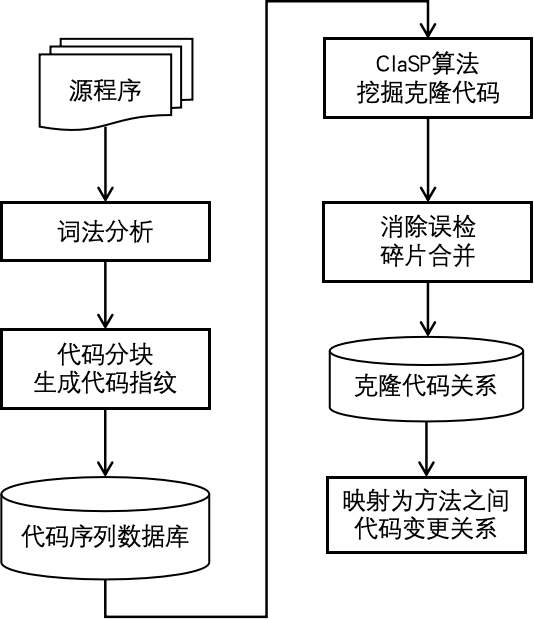
\includegraphics[width = 0.4\textwidth]{代码克隆流程}
\caption{基于代码克隆的变更影响分析方法流程}
\end{figure}



\subsection{代码预处理和分块}

为了精确有效地检测代码克隆,需先对源代码进行详细的预处理,以消除可能影响克隆检测准确性的各种干扰因素。

(1)代码标准化

首先,去除注释。注释通常用于解释代码的意图,并不直接影响程序的执行,但不同的代码实现中注释内容可能存在差异,这会导致本质相同的代码片段由于注释的不同而被误判为非克隆。因此,去除源代码中的注释是必不可少的步骤,它可以避免注释的差异干扰克隆检测的结果,从而确保算法专注于代码的实际逻辑。

接下来,去除头文件引用语句。在C/C++程序中,源代码文件往往会包含多个头文件,而不同的源文件可能引用相同的头文件。如果不对头文件进行统一的处理,算法就可能在不同的源文件中检测头文件引用的代码克隆情况,进而导致无谓的计算冗余。这不仅增加了处理的时间和空间复杂度,还可能影响克隆检测的效率和准确性。因此,合理的头文件处理可以有效地去除冗余,确保分析过程的高效性。

此外,考虑到代码克隆中的语法克隆类型,变量名的标准化处理在克隆检测中具有重要意义。具体而言,为了避免因变量名的变化导致漏检,在方法内部对变量名进行统一标准化处理,将所有局部变量和参数名替换为预定义的标准变量名,从而消除变量名不同带来的影响。这一过程有助于聚焦于代码的逻辑和功能层面,而非单纯依赖变量命名的差异,从而提高克隆检测的准确性和可靠性。

通过上述预处理过程,可以生成一个清晰、标准化的源代码文件,不仅消除了无关的噪声,还确保了源代码的逻辑和结构能够被准确捕捉,为后续的克隆检测提供了高质量的输入数据。

(2)代码分块

代码分块的主要目的是将代码拆解成更小、更易于对比的单元,从而提高克隆检测的准确性。本文的代码分块策略分为几步,首先对于基本语句,按固定行数分块,行数可由用户定义,默认为6行一块,行数越小则识别结果越精准,越能识别更细小的代码克隆情况。其次对于控制语句,识别并根据关键分块词(如 if, while, for, switch, try 等)进行分块,控制语句是代码逻辑的重要分界点,将它们作为分块的标准可以确保检测系统能聚焦于实际功能的逻辑边界。

此外,在代码克隆检测中,还需要遵循一些附加规则以确保检测的准确性和一致性。一是大括号不被视为代码块的一部分。这一处理策略是基于实际开发中的多样化书写风格所作出的考虑:不同的开发者在代码排版上可能存在差异,例如有的开发者将大括号置于同行,而另一些则习惯将大括号另起一行。为了避免这种格式差异对克隆检测结果产生干扰,大括号被排除在代码块之外,从而确保检测过程更侧重于代码的逻辑结构,而非视觉格式上的不同。二在分块过程中,为了便于后续的克隆检测和碎片合并,需要详细记录每个代码块的位置信息。这些信息通常包括:代码块所在的文件路径、代码块的起始行号和终止行号、代码块的总行数,以及每个块包含的具体行数。通过这种方式,不仅能够清晰地标识出每个代码块的位置,还能为后续的克隆碎片合并提供必要的上下文支持。

通过这些步骤和规则,代码被拆分成更小、更一致的单元,使克隆检测能够更加高效且精准地识别功能相似的代码块。

(3)代码指纹提取

这一步遍历代码块的每一行语句,将每行语句转化为数字序列,再将所有数字序列合并,转化为代码块的“指纹”。该指纹将代表代码片段用于识别代码片段之间的相似性或重复性。通过这种方式,不同的代码片段信息被压缩,转换为具有独特标识符的形式,从而在后续的分析中实现高效的比较和匹配。鉴于哈希算法在计算上的高效性与实现的简便性,它在生成代码指纹方面具有显著的优势。因此,本文选择采用冲突率较低的hashpjw算法提取代码指纹,以确保在保证高效性的同时,能够快速、准确地对代码进行相似性分析和重复性检测。


\subsection{基于代码克隆检测的变更影响关系提取}
序列数据挖掘(Sequence Data Mining,SDM)是时序数据挖掘领域的一个重要研究方向,旨在从给定的输入数据库中,探索在大量对象之间随时间频繁出现的模式。判断一个模式是否具有意义的阈值被称为最小支持度。SDM 已被广泛研究,并在多个领域得到了应用,如 DNA 序列中的基序发现、顾客购买序列分析、网页点击流分析等。本文中,将代码指纹片段作为序列,利用序列数据挖掘算法,挖掘频繁出现的模式,提取对应的代码克隆序列。

(1)数据挖掘领域基本概念

项集\cite{2013ClaSP}:设有一个集合 \( I = \{i_1, i_2, \dots, i_n\} \),其中 \( i_i \) 表示一个项。项集即为这个项的非空子集。一个项可以出现在多个项集中,但同一项集中的每个项只能出现一次,即不允许项集包含重复的项。在本文中,项集指的是代码行的指纹。

序列\cite{2013ClaSP}:序列是一个由项集组成的有序列表,记作 \( s = (s_1, s_2, \dots, s_n) \),其中每个 \( s_i \) 是项集。每个项集 \( s_i \) 可以进一步表示为 \( (x_1, x_2, \dots, x_m) \),其中 \( x_m \) 是项。本文中序列指代码块的指纹。

子序列\cite{2013ClaSP}:考虑两个序列 \( \alpha = (a_1, a_2, \dots, a_n) \) 和 \( \beta = (b_1, b_2, \dots, b_m) \),如果存在一组整数 \( 1 \leq j_1 < j_2 < \dots < j_n \leq m \),使得序列 \( (a_{j_1}, a_{j_2}, \dots, a_{j_n}) \) 是序列 \( \beta \) 的子序列,则称序列 \( \alpha \) 为序列 \( \beta \) 的子序列,序列 \( \beta \) 为序列 \( \alpha \) 的超序列。

序列数据库\cite{2013ClaSP}:序列数据库是由一组元组 \( \langle \text{sid}, s \rangle \) 构成的集合,其中 \( \text{sid} \) 为序列的标识符,\( s \) 为序列。如果序列 \( \alpha \) 是元组 \( \langle \text{sid}, s \rangle \) 中序列 \( s \) 的子序列,则称该元组包含序列 \( \alpha \)。序列数据库中包含序列 \( \alpha \) 的元组的数量被称为序列 \( \alpha \) 的支持度。本文中指的是项目代码所有分块的集合。

频繁子序列\cite{2013ClaSP}:给定一个正整数 \( \text{min\_support} \) 作为支持度阈值,如果序列 \( \alpha \) 的支持度大于或等于 \( \text{min\_support} \),则称序列 \( \alpha \) 为频繁子序列。所有频繁子序列的集合记为 \( FS \),即Frequent Subsequenc。


序列支持度:记作 \( \sigma(\alpha, D) \),是指在数据库 \( D \) 中包含序列 \( \alpha \) 的序列的总数。如果一个模式或序列至少出现给定的用户指定阈值 \( \text{min\_support} \),即最小支持度,则称其为频繁序列。频繁序列挖掘的问题就是在给定的输入数据库中,找到满足最小支持度阈值的频繁序列集合 \( FS \)。本文中即是找到频繁出现的代码。


闭合序列:如果一个频繁序列 \( \alpha \) 没有其他超序列与其具有相同的支持度,则称 \( \alpha \) 为闭合序列。所有频繁闭合序列的集合记作 \( FCS \)。更正式地说,若对所有 \( \beta \in FS \),有 \( \alpha \subseteq \beta \) 且 \( \sigma(\alpha, D) = \sigma(\beta, D) \),则 \( \alpha \in FCS \)。

闭合序列挖掘的问题就是在给定的输入数据库中,找到满足最小支持度阈值的闭合序列集合 \( FCS \)。显然,频繁闭合序列的集合要小于所有频繁序列的集合。这是因为在频繁模式的集合中,很多模式可能是冗余的。例如,某些频繁模式的支持度相同,且其中一个是另一个的超序列。对于这些模式而言,冗余的超序列模式没有提供比其子序列模式更多的信息。闭合频繁模式的引入可以去除这些冗余,保留那些最具代表性和信息量的模式。

这里举例说明,表3-1为序列数据库示例,这里设定最小支持度阈值为2。

\begin{table}[htbp]
\caption{序列数据库示例}
\vspace{0.5em}\centering\wuhao
\begin{tabular}{cccc}
\toprule
序列id(sid) & 序列 \\
\midrule
1 &  \langle (a)(ab)(bc)\rangle\\
2 & \langle (a)(abc) \rangle\\
3 & \langle (d)(a)(ab)(bc) \rangle\\
4 & \langle  (d)(ad)\rangle\\
\bottomrule
\end{tabular}
\end{table}

在这个例子中,第一个序列中有3个项集,分别是(a),(ab)和(bc),以此类推。根据上述概念计算得到,这个例子中的闭合频繁序列FCS=\(\{ \langle (a)\rangle, \langle (d)(a)\rangle, \langle (a)(ab)\rangle, \langle (a)(bc)\rangle, \langle (a)(ab)(bc)\rangle \}\), 共5个,而频繁序列有27个。因此识别闭合频繁模式具有重要的压缩性,并且模式信息也是不丢失的。

(2)ClaSP算法

ClaSP算法主要分为两步,首先生成频繁序列,作为频繁闭合序列的候选FCC(Frequent Closed Candidates)。第二步执行剪枝,从候选中剔除所有非闭合的序列,最终得到精确的FCS。主要的算法流程如3-1所示。

\begin{algorithm}
\caption{ClaSP算法}
\begin{algorithmic}
\KwIn{序列数据库}
\KwOut{频繁闭合序列集 $FCS$}
\State $F_1 \gets \{\text{频繁 1-序列}\}$ \\
\State $FCC \gets \emptyset$, $FCS \gets \emptyset$  \\
\For{\textnormal{all} $i \in F_1$} {
    \State $F_{ie} \gets \{\text{频繁 1-序列的长大于i的扩展序列 } \}$ \\
    \State $FCC_i \gets \text{DFS-Pruning}(i, F_1, F_{ie})$ \\
    \State $FCC \gets FCC \cup FCC_i$\\}
\EndFor
\State $FCS \gets \text{N-ClosedStep}(FCC)$
\end{algorithmic}
\end{algorithm}


首先找到所有的频繁的1-序列(即长度为1的序列),然后,对于所有频繁的1序列,递归地调用DFS-Pruning方法来探索相应的子树(通过进行深度优先搜索)。对所有频率为1的序列进行此处理,得到FCC,最后,算法结束去除FCC中出现的非闭合序列。


\begin{algorithm}[htbp]
\caption{DFS-Pruning算法}
\KwIn{当前模式 $p$, 候选项集 $S_n$ 和 $I_n$}
\KwOut{更新后的频繁模式集 $FCC$}

$Stemp \gets \emptyset$ 
$Itemp \gets \emptyset$ 
$F_i \gets \emptyset$ 
$P_s \gets \emptyset$ 
$P_i \gets \emptyset$ \\
\If{$\neg \text{checkAvoidable}(p, I(D_p))$}{
    \For{all $i \in S_n$}{
        \If{$p' = (s_1, s_2, \dots, s_n, \{i\})$ is frequent}{
            $Stemp \gets Stemp \cup \{i\}$ \\
            $P_s \gets P_s \cup \{p'\}$ \\
        }
    }
    $F_i \gets F_i \cup P_s \cup \text{ExpSiblings}(P_s, Stemp, Stemp)$ \\
    \For{all $i \in I_n$}{
        \If{$p' = (s_1, s_2, \dots, s_n \cup \{i\})$ is frequent}{
            $Itemp \gets Itemp \cup \{i\}$ \\
            $P_i \gets P_i \cup \{p'\}$ \\
        }
    }
    $F_i \gets F_i \cup P_i \cup \text{ExpSiblings}(P_s, Stemp, Itemp)$ \\
}
\Return{$F_i$} \\
\end{algorithm}
    

其中DFS-Pruning 算法的核心流程如3-2所示。通过递归生成候选模式(包括 s-扩展和 i-扩展,分别在模式末尾和任意位置添加新元素)并检查其支持度,最终返回以当前模式 $p$ 为前缀的所有频繁模式集。算法输入包括当前频繁模式 $p$ 以及用于执行扩展操作的候选项集 $S_n$ 和 $I_n$。

在 s-扩展阶段,算法遍历 $S_n$ 中的每个候选项 $i$,检查扩展后的模式是否为频繁模式。若为频繁模式,则将其加入 $Stemp$ 和 $P_s$ 中,并通过递归调用 ExpSiblings 方法继续扩展。i-扩展部分则类似,遍历 $I_n$ 中的候选项,检查并加入频繁扩展模式到 $Itemp$ 和 $P_i$ 中,最终进行 i-扩展的剪枝处理。

最终,算法返回以模式 $p$ 为前缀的所有频繁模式集 $F_i$,其中包括通过 s-扩展和 i-扩展生成的所有频繁模式。这些操作通过递归遍历模式树,确保高效地发现所有频繁模式。


剪枝时,通过检查对应模式的子序列和超序列的支持度,将序列的节点进行合并,防止继续遍历冗余节点。最终得到的FCS即为所有克隆代码集。

(3)合并碎片

由于先前的代码分段处理导致克隆代码呈现为片段间的克隆关系,为了恢复代码的完整性,进一步对这些碎片进行合并。具体而言,基于每段代码的位置信息,将属于同一方法的碎片进行合理整合,从而重建方法间的克隆关系。通过这种方式,最终得到的是方法与方法之间的克隆关系,反映了不同方法之间的相似性。

这种方法间的克隆关系不仅揭示了代码的重复性,还反映了不同方法之间在代码修改过程中的潜在影响。方法与方法之间的克隆关系可以被视为一种变更传播的路径,指示了某一方法的修改可能如何影响其他方法。因此,提取出的克隆关系即代表了方法之间的变更影响关系。

\section{基于数据挖掘的变更影响分析}
\subsection{代码变更历史提取}

在软件工程中,分析代码变更历史是理解软件演化重要手段之一。在开发者对项目进行维护的过程中,通常是以一个提交(commit)为单位进行功能上的变更。当进入新的维护工作时,如对同一功能进行升级等,通常的做法是参考前人的开发历史,对当前开发工作做指导,以防止变更的不完全。基于这一特点,本文设计了基于数据挖掘技术的变更影响分析方法,主要的挖掘对象是软件项目的变更历史。该方法能够全面地提取代码变更历史中的变更影响关系,尤其适用于具有丰富变更记录的软件项目。

该方法的核心假设是:在代码变更历史中,频繁同时更改的代码片段或方法对,通常存在着某种潜在的变更影响关系。这种变更影响关系不仅仅局限于语法上的依赖,还包括功能上的耦合和实现上的相互作用。因此,通过对这些历史变更数据的深入挖掘和分析,我们可以揭示出更深层的变更关系,为后续的代码优化、重构以及维护工作提供有力支持。

本方法的具体过程主要分为两部分,首先是对代码变更历史的收集与整理,然后通过数据挖掘技术提取并分析方法之间的变更影响关系。其中代码变更历史提取具体流程如下:

(1)收集项目代码库及变更历史记录

由于 Git 是现代软件开发中最广泛使用的版本控制工具,因此,本文的分析主要集中在 Git 项目上。首先,克隆项目的代码库到本地,项目中的.git文件夹中包含了版本变更历史记录,包括所有提交(commit)记录等。每个提交代表着代码库的一次变更,包含了代码的修改、删除或新增文件等信息。通过git log命令获取每次commit的详细信息,包括每个提交的哈希值、作者、日期和提交信息等。

(2)提取每个提交的变更信息

每个提交不仅仅是一个单一的代码变更,往往涉及多个文件的更改。因此,对于每个提交,运行git show <commitHash>命令,查看该提交引入的代码变更(即“diff”或差异),这会显示哪些文件被修改、添加或删除,本文主要关注标记为“修改”的文件,这些修改的文件中包含了具体的代码变化,即代码行的增、删、改操作,记录该commit引起的所有发生变更的代码行。

(3)定位变更代码行所属的方法

在提取了具体的代码变化后,定位这些变化的代码行所在的方法。通过libclang分析变化前文件得到的抽象语法树可获取每个方法对应的代码行,将变更的代码行的位置与方法位置进行匹配,进而得到变更的代码行所在的方法。

(4)提取变更方法与提交的关系

对于每个提交,提取出所有受影响的方法(即发生变化的方法),并将这些方法构成一个变更方法列表。这个列表反映了在特定提交中发生变更的所有方法,并为后续的变更影响分析提供了基础数据。用Map<commitID, List<Methods>>的结构存储每个commit变更的方法,作为序列数据库,便于后续分析与处理。


\subsection{基于共现关联挖掘的变更影响关系提取}

基于关联规则(Association Rules)的数据挖掘方法是反映事物之间相互依存性和关联性的一个重要数据挖掘技术,旨在从大量数据中挖掘出有价值的项之间的相关关系。共现关系可以视为关联规则的一种表现形式,它描述了在给定集合中,某一组项(或特征)经常出现在同一事务中。例如,在零售分析中,常见的共现关系是“购买了面包的顾客通常也会购买牛奶”。在这种情况下,“面包”和“牛奶”是一对共现项。

在本文的代码变更影响分析中,共现关系描述的是在一次提交中,哪些方法经常同时发生变更。如果两个方法在多个提交中频繁一起变动,则它们之间可能存在某种依赖关系或变更影响关系。通过分析这些方法在多个提交中被频繁同时修改的情况,我们能够识别方法之间的变更影响路径,从而揭示它们的潜在关联性。


常用的频繁项集的评估标准有支持度和置信度。支持度表示共现项在数据集中出现的次数占总数据集的比重,用于衡量一组项在数据集中的普遍程度。在代码变更分析中,支持度表示某一方法对在多个提交中同时出现的频率,计算公式如3-3.

\begin{equation}
Support(funcA,funcB)=\frac{num(AB\text{共现})}{num(AllCommits)}
\end{equation}

置信度表示共现项中一个出现后,另一个项出现的概率。变更分析中,置信度度量表示当方法A被修改时,方法B被修改的概率,计算公式如3-4。

\begin{equation}
Confidence(funcA\Leftarrow funcB)=\frac{P(AB\text{共现})}{P(B\text{出现})}
\end{equation}

在前文提取的序列数据库中,进行如下步骤的计算,详细流程见算法3-3。

首先,遍历序列数据库,搜索并得到候选 1 项集,即包含单个元素的项集,这些元素代表在变更历史中被修改过的方法。计算对应的支持度,剪枝去掉低于支持度的1项集,得到频繁1项集,频繁 1 项集中的元素反映了在变更历史中频繁出现的被修改方法。

基于频繁 1 项集中的元素,通过连接操作生成候选的频繁 2 项集。通过再次遍历序列数据库,计算候选频繁 2 项集的支持度,并筛选去除那些支持度低于设定阈值的项集。经过这一筛选步骤后,得到真正的频繁 2 项集。频繁 2 项集中的元素表示了那些在变更历史中频繁同时被修改的两个方法对。

在得到频繁 2 项集之后,进一步筛选出置信度高于或等于设定阈值的方法对。最终,留下的即为那些频繁同时变更,并且存在强关联关系的的方法对,表明它们在变更过程中有着较为显著的相互依赖关系,即方法对之间的变更影响关系。

\clearpage

\begin{algorithm}
\caption{变更影响方法对挖掘算法}
\begin{algorithmic}
\KwIn{序列数据库 $D$, 支持度阈值 $min\_sup$, 置信度阈值 $min\_conf$}
\KwOut{变更影响方法对 $change\_impact\_pairs$}
\State $F_1 \gets \emptyset$  \# 频繁1项集\\  
\For{all $f \in D$} {
    \If{support$(f) \geq min\_sup$} {
        $F_1 \gets F_1 \cup f$
    }
} \\
\State $F_2 \gets \emptyset$  \# 频繁2项集\\ 
\For{all $(f_1, f_2) \in P = \{ (f_i, f_j) \mid f_i, f_j \in F_1, i \neq j \}$} {
    \If{$\text{Support}(f_1, f_2) \geq min\_sup$} {
        $F_2 \gets F_2 \cup (f_1, f_2)$
    }
}

\State $change\_impact\_pairs \gets \emptyset$ \\ 
\For{all  $(f_1, f_2) \in F_2$} {
    \If{confidence$(f_1, f_2) \geq min\_conf$} {
        $change\_impact\_pairs \gets change\_impact\_pairs \cup (f_1, f_2)$
    }
}
\Return{$change\_impact\_pairs$}
\end{algorithmic}
\end{algorithm}
    
    



\section{基于深度学习的变更影响分析}

\subsection{数据集来源和收集}

当项目代码拥有丰富的变更历史时,可以通过前文中介绍的数据挖掘方法,提取具有变更影响关系的方法对。这种方法通过分析历史提交记录中方法间的共现频率,识别出在多次变更中相互依赖或相互影响的方法。然而,并不是所有软件项目都有变更历史可供我们分析,在仅有项目源代码的情况下,数据挖掘方法无法直接应用,但是只使用基于依赖闭包和基于克隆代码的方法,则无法识别除这两种关系外更深层次的变更影响。因此本文提出基于深度学习的变更影响分析方法,通过训练深度学习模型,对变更影响关系进行预测,以弥补另两种分析方法的不足。

为了识别那些来源除了依赖关系和代码克隆得到的代码变更影响关系,需要收集包含深层变更影响关系的方法对。而3.4节中根据数据挖掘的变更影响关系分析的方法,恰巧具有这一特征。该方法可以识别出那些在多个提交记录中频繁同时发生变更的方法对,由于我们的标准设置十分严格,因此识别的变更影响关系具有较强的可靠性,可作为数据集的正例进行收集。此外,为了构建平衡的数据集,通过对项目中的方法进行随机抽样,从中选取一些不具有变更影响关系的方法对,作为数据集的负例进行收集。

在数据集收集过程中,本文面临了几个挑战。首先,一些看似活跃的项目(例如频繁提交的项目)实际上并未挖掘到大量可用数据。分析原因是由于项目规模较大,文件数量庞大,开发者的工作内容往往不具有交集,大部分的方法不会被二次更改,因此难以出现频繁的样例。其次,对于一些发展时间较长的项目,因为提交记录众多(如数万次提交),所以在收集数据时需要处理大量的提交,这使得数据处理的过程非常耗时。

为了解决这些问题,本文在选择项目时设定了一些标准。首先,优先选择规模适中的项目,这些项目既足够活跃,又不会因为过于庞大的代码库而导致数据处理困难。同时,考虑到提交记录较多的项目可能导致数据量过大,本文限制了采集范围,只选择了最近的提交记录(例如最新的10000个提交)。这一策略有两个主要考虑:一方面,确保数据量足够大,以支持后续的挖掘工作;另一方面,聚焦于那些近期频繁变动的方法,排除较为稳定且变化较少的旧函数,从而更好地反映出当前项目的活跃度和变更趋势。

最终本文选择了基于表 2-1 中列出的GitHub项目。这些项目除了符合上述条件外,还有以下优点。首先,它们的收藏数均在千以上,表明这些项目在开源社区中具有较高的关注度和影响力,并且被广泛使用。其次,这些项目的社区非常活跃,说明项目持续更新和迭代,保证了具有较为丰富的变更历史,能够为我们的变更影响关系分析提供丰富的数据支持。

\subsection{基于代码预训练模型的变更影响关系预测}

基于深度学习的影响关系预测任务的输入为两个方法体,输出为两个方法之间存在变更影响关系的概率,概率越接近 1,表明这两个方法之间有关系的可能性越大。

考虑到代码理解的复杂性与深度,本文采用了基于预训练模型的代码表示学习方法,选择了 CodeBERT 作为核心模型。CodeBERT 是一种专为程序代码设计的预训练语言模型,通过大规模的代码语料库预训练,能够学习到代码中的丰富语法结构和语义信息。经过 CodeBERT 模型的表示学习,所得到的向量不仅包含了每个方法体的语法特征,还能够编码代码中的语义关系及其他潜在的编程特征。模型架构如图3-3所示。

\begin{figure}[h]
\centering
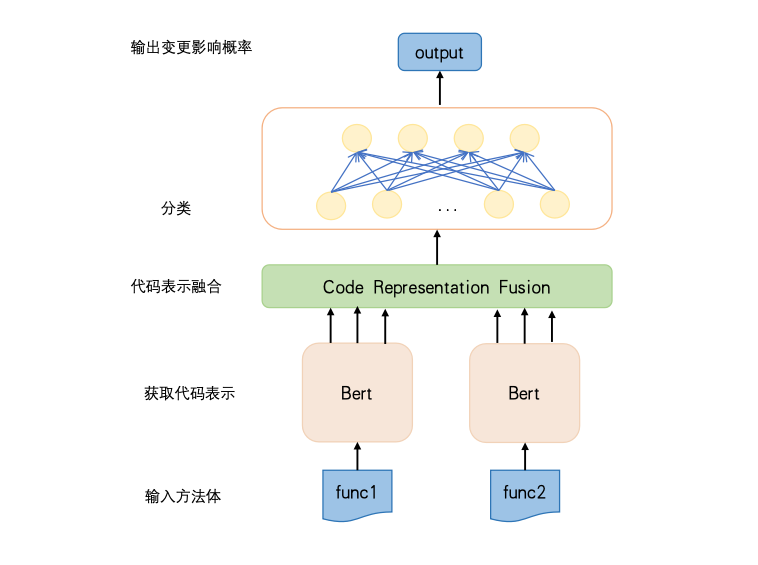
\includegraphics[width = 0.8\textwidth]{模型架构3.jpg}
\caption{基于代码预训练的深度学习模型架构}
\end{figure}


首先,将两个方法体$ F_a, F_b$,先通过代码预训练模型进行编码

\begin{align}
H_a=&Encoder(F_a) \in \mathbb{R}^{(len,dim)} \\
E_a=&mean(H_a[1:...]) \in \mathbb{R}^{(dim)}
\end{align}

得到方法的向量化表示$ E_a, E_b$,通过拼接融合这两个向量,将融合后的向量表示送入一个由两层组成的多层感知机(Multilayer Perceptron,MLP)中,再通过 softmax 层进行分类处理,将模型的输出转化为一个概率分布,表示两个方法体之间存在关系的概率。

\begin{align}
E_{a,b}=Concat(E_a,E_b)& \in \mathbb{R}^{(dim*2)} \\
logits_{a,b}=MLP(E_{a,b})&=FFN(ReLU(FFN(E_{a,b}))) \\
FFN(x)&=Wx+b\\
ReLu(x)&=max(0,x)\\
logits_{a,b}& \in \mathbb{R}^{(2)}
\end{align}

最后与真实标签计算交叉熵损失,得到loss,计算梯度,优化模型参数
\begin{align}
loss=CrossEntryLoss(logits_{a,b}, Label)
\end{align}

\section{实验结果与分析}

\subsection{实验数据集描述}

本章依旧使用表2-2的示例项目进行研究。基于深度学习的变更影响分析方法的数据集收集方式如3.5.1节所述。数据集统计信息如表3-2所示,共7351对数据,按照训练、验证、测试集 为 6:2:2 进行训练和测试。这里排除了antiword项目,因为该项目并没有官方维护的github仓库,因此无法获得足够的历史变更。

\begin{table}[htbp]
\caption{数据集统计信息}
\vspace{0.5em}\centering\wuhao
\begin{tabular}{cccc}
\toprule
项目名称 & 正例对数 & 负例对数 & 总对数 \\
\midrule
TheAlgorithms & 110 & 1000 & 1110 \\
jemalloc-5.3.0 & 641 & 1000 & 1641 \\
libbpf-1.1 & 418 & 1000 & 1418 \\
librdkafka-2.1.0 & 1164  & 1000 & 2164 \\
FFmpegKit-5.1.0 & 18 & 1000 & 1018 \\ 
总计 & 2351 & 5000 & 7351 \\
\bottomrule
\end{tabular}
\end{table}

\subsection{实验设置与评价方式}
1. 实验设置

(1)深度学习实验设置

针对基于深度学习的变更影响分析方法。本文使用了CodeBERTa-small-v1和codebert-base-mlm两个模型分别作为代码表示学习模型,得到的代码表示为768维,融合时使用的MLP的每层维数为(768*2,64,2)。

模型的参数设置如表3-3。

\begin{table}[htbp]
\caption{模型参数设置}
\vspace{0.5em}\centering\wuhao
\begin{tabular}{cccc}
\toprule
超参数 & 数值  \\
\midrule
Token embedding size & 768 \\
codeBERT learning-rate  & 1e-5 \\
codeBERT dropout & 0.4 \\
Classifier learning-rate& 1e-4 \\ 
Adam \beta_1  & 0.95  \\
Adam \beta_2 & 0.999  \\
batch\_size & 64 \\
\bottomrule
\end{tabular}
\end{table}

(2)基于数据挖掘方法实验设置

本文将置信度设置为1。具体而言,对于方法A,记录其在所有提交记录中出现的次数为\(N_A\),并统计在这些提交中,其他方法B出现的次数为\(N_B\)。如果在所有提交中,方法A出现时,方法B的出现频率达到\(N_A \backslash N_B = 1\)
则认为方法对 $(A, B)$ 存在变更影响关系。换句话说,置信度为1表示每当方法A被修改时,方法B也必然随之修改,从而确认这两个方法的变更是紧密关联的,并且它们的修改行为是同步的。

本文将支持度设置为2和3分别进行实验,意味着方法A和方法B在多个提交中同时出现的次数必须至少为2或3次,才能认为这两个方法之间可能存在变更影响关系。支持度的设定要求方法对 $(A, B)$ 在变更历史中有一定的共现频率,从而能够确保所识别的变更影响关系具有一定的统计显著性,避免偶然性因素的干扰。通过对比2和3,研究支持度的不同对于实验结果的影响。

2. 评价方式

本章的评价指标主要分为两部分,第一部分的评价指标如式(3-13)(3-14)(3-15)所示,在表2-2的每个示例项目中,随机选取20个方法进行变更,人工分析其变更得到实际的被影响方法AIS(Actual Impact Set),每种方法计算得到估计的被影响方法EIS(Estimated Impact Set),根据这两个值计算精确度、召回率和F-measure,这三种评价指标在信息检索的场景下被广泛使用,本章中用于评价变更影响分析方法的有效性。
\begin{equation}
{precision} = \frac{|EIS \cap AIS|}{|EIS|}
\end{equation}

\begin{equation}
{recall} = \frac{|EIS \cap AIS|}{|AIS|}
\end{equation}

\begin{equation}
F-measure = \frac{2 \times precision \times recall}{precision + recall}
\end{equation}

除了验证变更影响分析方法的有效性外,还需要将分析得到的变更影响关系与代码质量相结合,以便向用户提供更具参考价值的质量报告。一般而言,一个成熟且高质量的软件项目通常具有清晰的模块化结构,体现出高内聚、低耦合的特性,因此维护起来会更加方便。从更具体的角度来看,对于一个方法而言,如果它的变更会影响到较大的范围,这可能表明软件架构存在问题,内聚性不足,耦合度较高,从而导致较差的可维护性。

基于上述分析,本章进一步统计了变更影响关系数量位于前 5\% 的方法,认为这些方法可能是代码质量较差的特征代表,并将其作为重点信息报告给用户。通过这种方式,用户能够快速定位系统中可能存在维护隐患的关键方法,从而更有针对性地优化系统设计和提高软件质量。

第二部分评价方式与第二章中所述相同。对报告的质量较差的方法进行统计,计算用户接受率作为主要指标,具体的计算公式可参见式(2-9)。接受率作为衡量实验效果的重要标准,有助于评估系统在实际应用中的表现和用户的反馈。然而,仅依赖上述评价指标可能无法全面反映实验的真实情况,因此,为了确保实验结果的可信度与全面性,本研究还进行了大量的实例分析和统计分析。

\subsection{实验结果与实例分析}

本节将通过实验对比来评估本章提出的三种变更影响分析方法的性能,这里主要讨论下列三个问题:

RQ1:本章节提出的三种方法能否有效地提取变更影响关系?与现有方法相比,它在F-measure、召回率和精确率的表现如何?

RQ2:这三种方法各自的优势如何?分别适用于哪些特殊场景?又各自有怎样的局限性?

RQ3:这三种方法检测到的变更影响关系对软件项目的质量贡献如何?应从什么角度指导开发者对软件项目进行维护?

\textbf{1.针对于RQ1的实验}

为了评估本章提出的方法在检测依赖型和逻辑型的变更影响关系的性能,本文实现了基于传递依赖闭包的方法,并与本章提出的三种方法进行了对比实验。结果如表3-4所示。通过实验结果可以发现,不同方法在变更影响分析中的表现各有侧重。

\begin{table}[htbp]
\caption{变更影响实验结果 - F-measure/召回率/精确度}
\vspace{0.5em}\centering\wuhao
\begin{tabular}{ccccc}
\toprule
方法 & F-measure & recall & precision  \\
\midrule
依赖闭包 & 43.9 & 75.6 & 30.9 \\
克隆代码 & 3.7 & 1.9 & \textbf{95.0} \\
数据挖掘 & \textbf{75.1} & \textbf{87.3} & 65.9\\
深度学习 & 54.9 & 69.6 & 45.3 \\
\bottomrule
\end{tabular}
\end{table}

首先分析传统依赖闭包方法,通过实验结果可以发现,该方法的召回率较高为75.6\%,说明它能够识别大部分的变更影响关系,即大部分真正的变更影响关系被识别了。然而其精确率较低,仅为30.9\%,是所有方法中精确率最低的,这说明该方法的识别结果中存在大量的误报,即大量没有变更影响关系的方法被其误认为有影响关系。这正是由于依赖闭包方法本身的特性决定的,由于变更影响关系随涟漪扩散效应,越向外扩散影响越小,但该方法却平等地认为扩散所至的代码均存在影响关系,这不符合扩散效应的特性。如在图3-4中所示是antiword项目中从bTranslateImage方法出发得到的调用图,它完整地体现了从word中提取jpec图片的过程,bTranslateImage调用bTranslateJPEG,处理jpec图片,再调用vASCII85EncodeFile,将图片提取为文件,再依次调用vASCII85EncodeArray和vASCII85EncodeByte,层层处理直到完成对图片的提取(后文使用后缀代指)。当对Byte方法进行变更影响分析时,根据RETURN关系的涟漪扩散效应,最终会将图中所示的其他4个方法都列为会受到变更影响的方法。然而实际上,该方法只对\{Array, File\}存在变更影响关系,当Byte方法的签名发生改变时,将直接影响到\{Array, File\},这两个方法如果不更改将发生编译错误。而对另两种方法的影响则微乎其微,化为了动态运行时内部值的变化,实际上不一定会真的产生影响。

\begin{figure}[h]
\centering
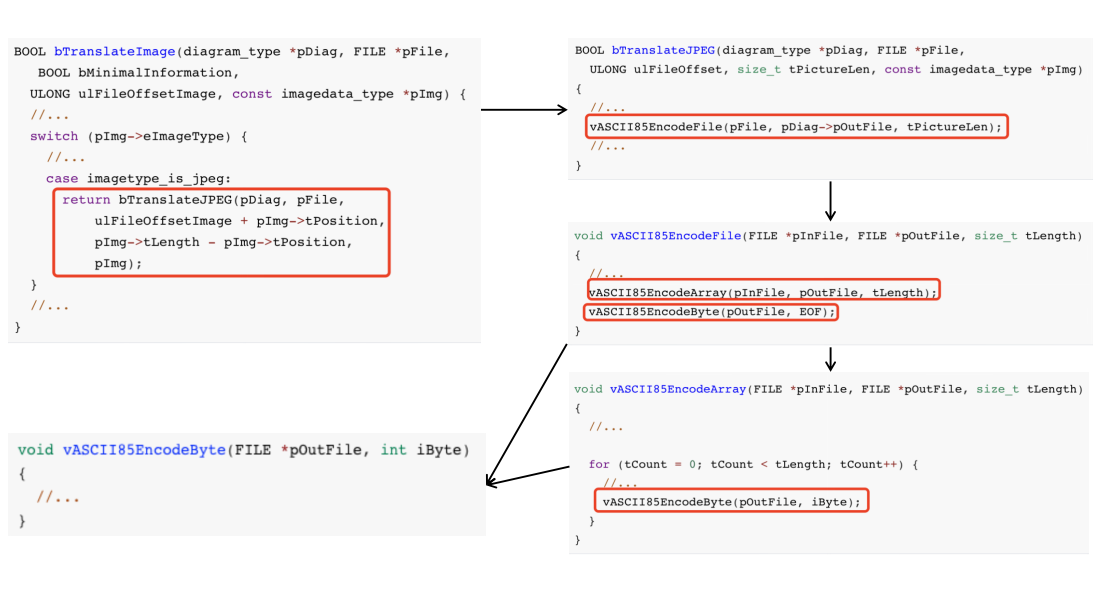
\includegraphics[width = 1\textwidth]{静态分析拒绝样例.jpg}
\caption{依赖闭包方法被用户拒绝实例}
\end{figure}

对基于克隆代码的方法进行分析,该方法展现的实验结果最为特殊,其精确率最高,这说明其识别的正例非常准确,很少出现误报的现象。但是它的召回率极低,表明该方法对大部分的变更影响关系无法识别到,这是由于在项目中,大部分的变更影响关系为依赖型,而克隆代码只是逻辑型的一种,因此提取到样例本身也较少,就导致其整体效果不佳。

基于数据挖掘的方法表现最好,其F-measure在所有方法中表现最优。这表明,代码变更历史中的确蕴含了大量能够有效揭示变更影响关系的信息,这是因为变更历史中都是前人对软件项目进行变更的记录,这样的提交由开发者精确变更,并经历过开源项目中非常严格的审查过程才合入主分支,因此较为准确地反映了代码变更中的实际操作,从而也能将过去的开发模式反映在数据挖掘的结果集中。

而基于深度学习的方法则略差于基于数据挖掘的方法,有一定的误报和漏报,但总体上来说优于依赖关系闭包和克隆代码的方法。这表明深度学习方法能够在数据集中较为有效地学习在开发者在变更过程中展现的行为模式,并迁移到新的方法判断中。


\textbf{2.针对于RQ2的实验}

RQ1中从整体的角度上说明了三种方法的有效性。为了回答RQ2中三种方法的优势,这里对每种方法检测得到的依赖型和逻辑型的变更影响关系分别进行统计为表3-4,其中EIS表示估计影响集的数量,即方法预测得到的变更影响集的数量,而AIS表示实际影响集的数量。

\begin{table}[htbp]
\caption{变更影响实验结果}
\vspace{0.5em}\centering\wuhao
\begin{tabular}{ccccc}
\toprule
方法 & 依赖型EIS & 逻辑型EIS & 依赖型AIS & 逻辑型AIS  \\
\midrule
依赖闭包 & 2446 & 0 & 756 & 0 \\
克隆代码 & 0 & 20 &  0 & 19 \\
数据挖掘 & 914 &  410 & 499 & 375 \\
深度学习 & 861 & 675 & 421 & 275 \\
\bottomrule
\end{tabular}
\end{table}

对每种方法检测的关系数量进行归一化,排除检测数量对结果分析的干扰,绘制如图3-5所示的条形图。其中同一方法内浅色柱的对比表现了该方法在检测时的报告关系比例,说明其倾向和检测类型的能力。而深色柱则表明了对应报告类型的准确率,说明其性能。以依赖闭包方法为例,其检测到的关系均为依赖类型,而报告的准确率达到30.9\%,这表明该方法仅能检测依赖型方法,且误报率较高。以此类推可进一步分析其他方法的类型检测能力及准确性。


\begin{figure}[h]
\centering
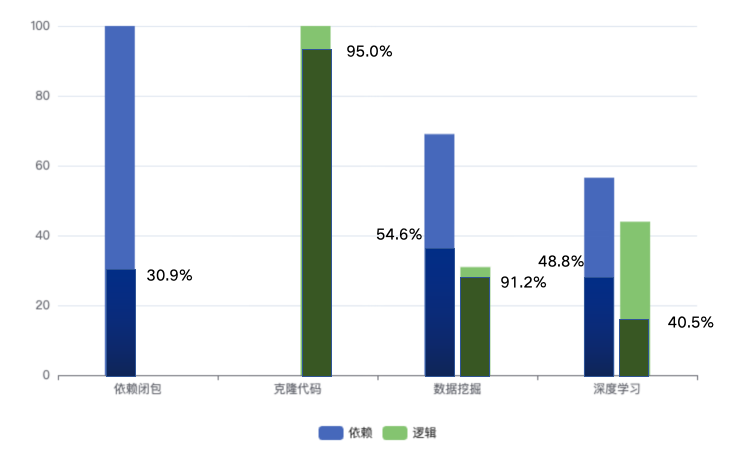
\includegraphics[width = 0.8\textwidth]{倾向与正确率.jpg}
\caption{依赖闭包方法被用户拒绝实例}
\end{figure}


基于克隆代码的方法仅能检测逻辑型的变更影响关系,但是其准确率能达到95\%。结合RQ1中的分析结果,这表明基于克隆代码方法非常擅长挖掘逻辑型中由于克隆代码导致的变更影响关系。图3-6为克隆代码方法挖掘到的一对有变更影响关系的方法。这里展示了这对方法的部分代码,其中绿色高亮的部分表示代码克隆的区域。这两个方法的主要功能是分别对8位和4位压缩格式的图像进行解码。我们发现,这对方法中的大部分逻辑结构几乎完全相同,只有少部分关键处理逻辑存在差异。由此,我们可以认定,这两个方法的变化过程很可能是同步的,即在实际的维护过程中,当对其中一个方法进行修改时,另一个方法也通常需要同步进行相应的变更,才能保证逻辑的一致性。

\begin{figure}[h]
\centering
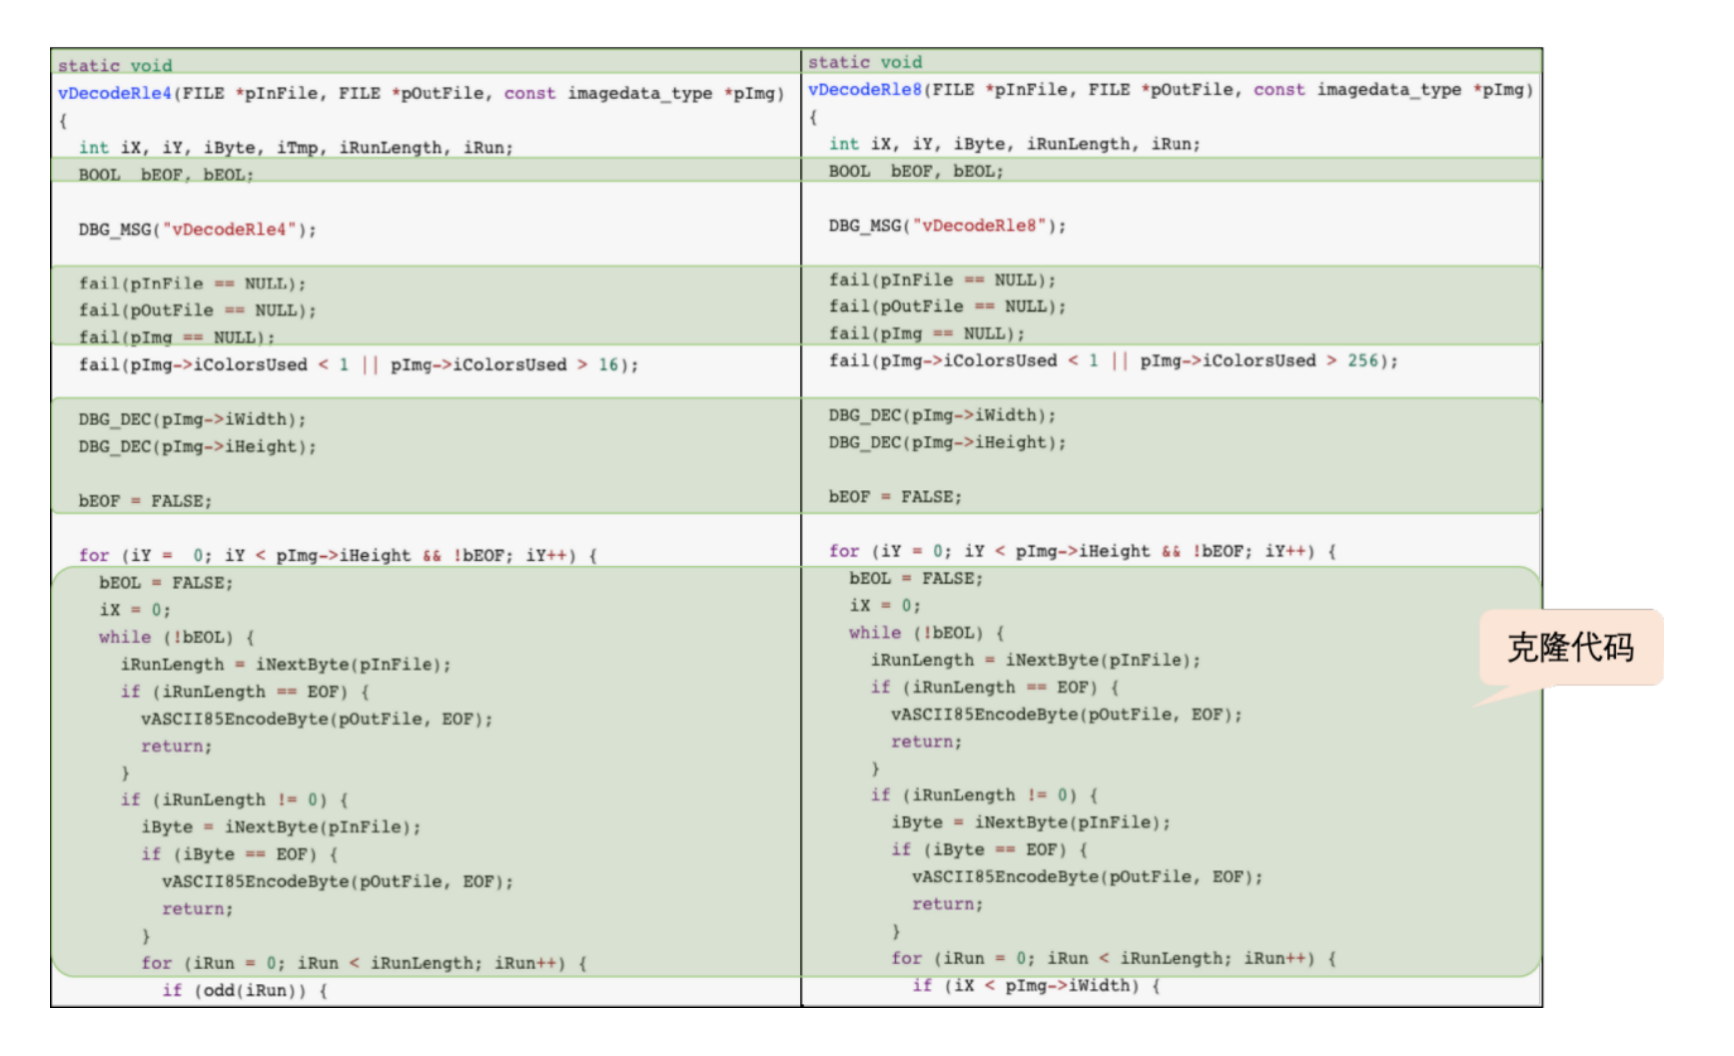
\includegraphics[width = 1\textwidth]{克隆代码示例.jpg}
\caption{包含克隆代码片段的一组方法实例}
\end{figure}

这种代码克隆现象表明,在软件的演化过程中,维护人员可能需要对这两个方法进行联动更新。任何对其中一个方法的修改都可能影响到另一个方法的功能或逻辑一致性,因此在代码维护时,特别是针对这类高度相似的方法,必须考虑它们之间的相互依赖关系。这种潜在的同步更新要求在进行变更影响分析时,尤其是在代码质量评估和变更影响分析的研究中,必须给予充分的关注,以确保系统的稳定性和一致性。

基于数据挖掘的方法可以挖掘两种类型的变更影响关系,根据报告比例,可以发现其报告依赖型更多,这是由于对于质量良好的项目来讲,通常项目中的依赖型变更影响关系更多,能够通过编译器或开发工具即可让开发者掌握项目架构。除此之外该方法对于逻辑型的关系更为擅长,表现为在挖掘到的逻辑型关系中,准确率能达到91.2\%,而对于依赖型的变更影响,则同样存在误报的情况,根据方法的设计思路,推测这里是由于在项目早期,开发者人数较少,项目发展较快,变更较频繁,所以通常都是大量代码一起提交并且频繁更改造成的偶然现象,未来或许可通过仅挖掘项目稳定后的变更历史来改善。

为了说明数据挖掘方法的优秀潜力,以 librdkafka 项目中挖掘到的一对方法为例,该项目是 Apache Kafka 的一个高性能 C/C++ 客户端库。图 3-7 展示了通过数据挖掘技术发现的一对存在变更影响关系的方法。左侧的方法rd\_kafka\_global\_cnt\_decr负责对计数器进行减一操作,而右侧的方法rd\_kafka\_global\_cnt\_incr则负责对计数器进行加一操作。

\begin{figure}[h]
\centering
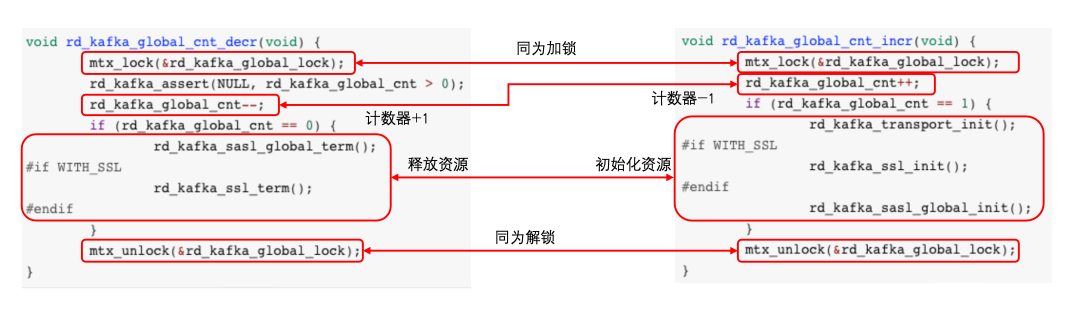
\includegraphics[width = 1\textwidth]{incrdec.jpg}
\caption{逻辑上有变更影响关系的方法对示例-incr和decr}
\end{figure}

从功能上来看,这两个方法是一对典型的协作方法,其作用密切相关。具体来说,incr方法不仅执行计数器加一操作,还在计数器从零变为一时,执行资源的初始化工作,确保所需资源在后续操作中可用。而 decr方法则在计数器减为零时,执行资源的释放操作,以清理不再使用的资源,避免资源泄漏。从代码实现可以看出,这两个方法的操作逻辑具有明显的互补性,加一与减一、初始化与释放的功能关系呈现出“镜像”特性。

尽管它们在代码中并未直接相互调用,也未调用相同的函数,但由于它们在功能上承担了计数器的管理和资源的初始化与释放工作,其逻辑关联性非常强。因此,当其中一个方法的实现逻辑发生变化时,另一个方法通常需要进行相应的调整,以保持整体逻辑的一致性。这种方法对的变更影响关系属于典型的逻辑关联型变更影响关系,而非通过直接调用或共享资源显式连接的变更关系。这种逻辑上的关联性表明,数据挖掘方法能够有效捕获代码中隐性的、非显式的变更依赖。

\begin{figure}[h]
\centering
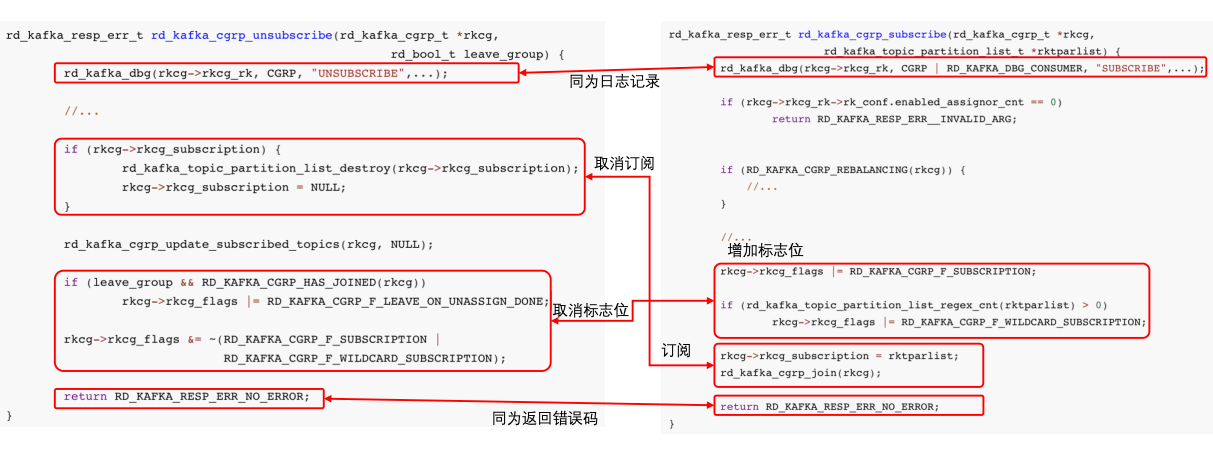
\includegraphics[width = 1\textwidth]{subscribe.jpg}
\caption{逻辑上有变更影响关系的方法对示例-subscribe和unsubscribe}
\end{figure}

图3-8所示是一个更加复杂的例子,这个例子同样是一对有逻辑关联型变更影响关系的方法。这对方法的功能分别是对 Kafka 的主题(topic)进行订阅和取消订阅。左侧的方法负责实现对指定主题的取消订阅操作,而右侧的方法则负责实现订阅操作。尽管这两个方法在代码上并未直接相互调用,但它们在逻辑上具有显著的关联性,尤其是在处理订阅状态的管理上,在订阅操作中,方法会新增订阅标志位、更新订阅的主题列表。而在取消订阅操作中,方法会移除对应的订阅标志位、清空订阅列表,并在必要时清理与订阅相关的组资源。这种逻辑上的互补关系,使得订阅和取消订阅操作形成了一个完整的管理闭环。

从功能视角来看,订阅和取消订阅的行为本质上是对同一资源或逻辑状态的不同操作。这种镜像特性意味着,当订阅逻辑发生变化时,例如新增了订阅标志位的更新规则或修改了主题列表的处理方式,取消订阅逻辑通常也需要进行相应的调整,以保证订阅状态管理的完整性和一致性。

这两对方法体现了典型的逻辑关联型变更影响关系。这种关系不同于通过显式调用或共享资源产生的直接依赖,而是一种通过功能和逻辑流程相互关联的隐性依赖。这种实例表明,即使在方法间没有显式的代码关联,数据挖掘方法仍能够捕获这类隐性逻辑关联,为代码变更影响分析提供了有力支持。通过识别这类方法对,开发者在维护和演化代码时可以更好地理解潜在的影响范围,避免遗漏可能的关联性调整,提高系统维护的可靠性和效率。


基于深度学习的方法在数据集上的实验结果如表3-5所示,从总体上来看,两个模型的性能均表现出色,深入分析可以发现两个模型各有所长。

\begin{table}[htbp]
\caption{基于代码预训练模型的变更影响关系预测实验结果}
\vspace{0.5em}\centering\wuhao
\begin{tabular}{cccc}
\toprule
模型& F-measure & recall & precision \\
\midrule
CodeBERTa-small-v1 & 91.8 & 86.1 & 98.2 \\
codebert-base-mlm  & 87.1 & 100.0  & 77.1 \\
\bottomrule
\end{tabular}
\end{table}

CodeBERTa-small-v1 模型更强调预测出的正例的真实性和准确性。这意味着它在确保预测结果的准确性方面做得很好,但可能会导致一些正确的情况被漏掉,即存在漏报。此外由于"small"模型的规模较小,参数数量较少,这可能会使得模型在训练过程中更容易发生过拟合现象。而CodeBERT-base-mlm 模型则更注重捕捉尽可能多的正样本。这个模型虽然能够覆盖更多的正例,但也引入了更多误报。但是该模型参数更多,具备更强的泛化能力,通常能够更好地适应新的数据集。

深度学习方法在实际应用中的效果如图3-5中所示,其可以挖掘两种类型的变更影响关系。与数据挖掘方法相比,该方法更倾向于挖掘逻辑型变更影响关系,表现为逻辑型报告比例相较于数据挖掘方法更多,这或许是由于数据集的不平衡所导致的。尽管两种类型的准确率均不高,但仍能从检测出的样例中发现一定的实际应用价值,在没有代码变更历史的软件项目中,可以作为对传统方法的补充。



接下来对对支持度不同的实验结果进行分析。可以发现,支持度为3略高于支持度为2的接受率,这是由于,支持度为3意味着这对方法起码发生共同修改三次才能被挖掘到,这排除了共同修改2次的方法对的一些偶然情况,挖掘到的关系更少,但是也更为精准。因此,支持度也是决定数据挖掘方法精确度的重要因素之一。


\textbf{3.针对于RQ3的实验:}

统计用户的接受率。得到的结果如表3-5所示。

\begin{table}[htbp]
\caption{变更影响实验结果-接受率}
\vspace{0.5em}\centering\wuhao
\begin{tabular}{ccccc}
\toprule
项目名称 & 依赖闭包 & 克隆代码 & 数据挖掘-支持度2 & 数据挖掘-支持度3 \\
\midrule
TheAlgorithms & 36.2 & 92.3 & 81.2 & 89.4\\
antiword-0.37 & 33.7 & 89.9 & - & -\\
jemalloc-5.3.0 & 33.4 & 89.3 & 69.8 & 92.1\\
libbpf-1.1 & 40.4 & 94.4 & 76.4 & 77.3\\
librdkafka-2.1.0 & 28.3 & 83.7 & 74.3 & 83.2\\
FFmpegKit-5.1.0 & 27.2 & 84.7 & 64.7 & 87.0\\

\bottomrule
\end{tabular}
\end{table}

(1)基于依赖关系闭包的方法

进一步对基于依赖闭包的方法的实验结果进行实例分析,本方法接受率最低,究其原因可以发现这是由于依赖闭包这个方法本身的特性决定的。这个方法实际上依靠的是变更的涟漪效应,而这种效应越向外扩展则影响越小,影响越小则用户越难以分辨其是否会产生真正的变更影响。

,并且说明了与用户对变更传播的认知高度契合,进一步验证了本文假设:克隆代码一定程度上反映了变更影响关系。


除此之外,我们还观察到部分未被接受的方法对存在一些特定的特征,进一步揭示了影响用户接受率的其他因素。例如,以antiword项目中的一对包含克隆代码片段的方法为例,这两个方法的统计信息如表3-6所示,其中克隆代码片段仅占据8行。代码长度的可视化形式以及克隆代码片段如图3-6所示,包含的重复代码仅为两行单独的语句。之所以在统计时被视为克隆代码,主要是由于编程习惯的影响,每个参数被单独放在一行,这导致了克隆代码的扩展至8行。用户认为此例较为牵强,因为克隆代码占整个方法的行数过少,这表明克隆代码所占比例可能是用户决定是否信任该项分析的重要因素之一,除此之外这一点可能也需在对代码进行预处理时,对代码格式进行统一,防止一句扩展成多行的情况发生。

\begin{table}[htbp]
\caption{被用户拒绝实例代码信息}
\vspace{0.5em}\centering\wuhao
\begin{tabular}{cccc}
\toprule
方法 & 代码行数(Line of code)  & 克隆代码长度\\
\midrule
pHdrFtrDecryptor & 125 & 8 \\
szFootnoteDecryptor  & 115 & 8 \\
\bottomrule
\end{tabular}
\end{table}

\begin{figure}[h]
\centering
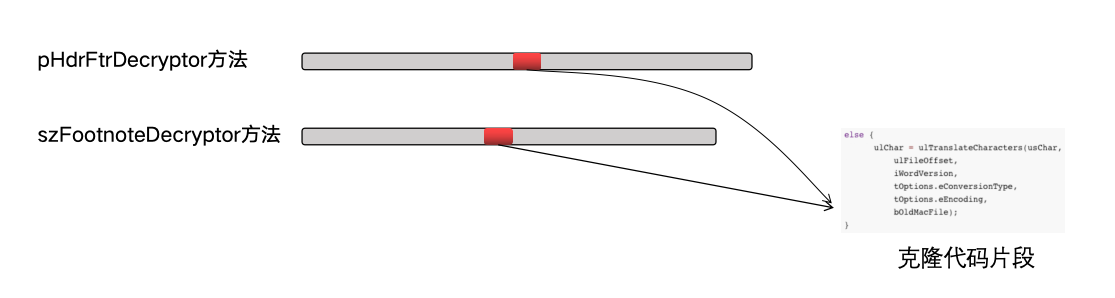
\includegraphics[width = 1.0\textwidth]{克隆代码拒绝样例.jpg}
\caption{被用户拒绝实例代码长度可视化}
\end{figure}


3. 变更影响分析方法总结

总的来说,本文提出的三种方法均从不同角度弥补了传统基于依赖传递闭包方法的不足,为代码变更影响关系的检测提供了多样化的解决方案。这些方法各有侧重,适用于不同的应用场景,同时也具有一定的局限性。总结如下:

首先,基于克隆代码的方法专注于逻辑型变更影响关系中的代码克隆检测。这种方法尤其适用于由于代码克隆导致的变更影响关系场景,其优势在于检测结果的精确性,能够准确捕捉代码克隆带来的变更传播。然而,其局限性在于检测范围仅限于代码克隆这一种关系,无法适应其他类型的变更影响。

其次,基于数据挖掘的方法能够同时覆盖依赖型和逻辑型变更影响关系,适用于具有丰富代码变更历史的项目。通过挖掘项目中隐含的变更模式和历史记录,该方法可以捕获更多类型的变更影响。然而,对于没有变更历史或变更频率较低的项目,这种方法可能失去其效果,限制了其广泛应用的场景。

最后,基于深度学习的方法同样能够检测依赖型和逻辑型变更影响关系,尤其适合没有变更历史的项目。这种方法通过预训练模型的泛化能力,能够在缺乏历史数据的情况下预测变更影响。然而,其不足之处在于对训练数据质量的高度依赖,数据不完整或质量不高可能直接影响检测结果的可靠性。

\begin{table}[htbp]
    \caption{基于代码预训练模型的变更影响关系预测实验结果}
    \vspace{0.5em}\centering\wuhao
    \begin{tabular}{ccp{4cm}p{4cm}}
    \toprule
    方法& 检测关系 & 适用场景 & 缺点\\
    \midrule
    克隆代码 & 逻辑型中的代码克隆 & 由于代码克隆导致的变更影响关系 & 只能检测代码克隆一种关系\\
    数据挖掘  & 依赖型和逻辑型 & 有代码变更历史的项目 & 无法应用于没有变更历史的项目,如果不频繁变更可能无法被检测 \\
    深度学习  & 依赖型和逻辑型 & 没有变更历史的项目 & 依赖于训练数据的质量 \\
    \bottomrule
    \end{tabular}
    \end{table}

综上所述,这三种方法在各自的适用领域内展现出了显著的优势,同时也存在一定的局限性。通过结合这些方法,可以为代码变更影响分析提供更全面的支持,满足不同场景下的需求,从而提升系统维护与演化的效率与质量。

\section{本章小结}

本章介绍了四种变更影响分析方法。首先是传统的基于依赖关系闭包的变更影响分析方法。该方法首先对软件项目进行预处理,提取抽象语法树、方法摘要表和全局变量信息表等数据结构,然后构建依赖关系图,节点表示方法和全局变量,边表示方法之间的调用关系。然后根据依赖闭包对每个方法提取对应影响方法。其次是基于克隆代码的变更影响分析方法。该方法认为代码克隆关系一定程度上反映了变更影响关系,通过ClaSP算法进行序列挖掘,提取代码克隆,从而反映变更影响关系。第三种是基于数据挖掘的变更影响分析方法。该方法认为代码变更历史蕴含了一定的变更影响关系,通过提取代码的提交历史,根据频繁模式挖掘理论,挖掘出频繁共现的方法对,从而反映变更影响关系。第四种是基于深度学习的变更影响分析方法。对不存在变更历史的项目,通过数据挖掘得到的数据整理成数据集,训练深度学习模型,对项目方法之间的变更影响关系进行预测。最后,本章通过实验验证了四种方法在提取变更影响关系上的有效性,实验结果表明,除传统的基于依赖关系闭包的方法外,其他方法都取得了良好的检测效果。除此之外还通过实例分析,说明了每种方法的缺点和各自的侧重点。

%%%%%%%%%%%%%%%%%%%%%%%%%%%%%%%%%%%%%%%%%%%%%%%%%%%%%%%%%%%%%%%%%%%%%%%%%%%%%%%


\chapter{基于代码审查图的代码架构和质量信息可视化}
\section{引言}


在软件开发过程中,开发者通常会经历多个阶段。在项目的初始阶段,开发者需要阅读和理解已有的代码,这是熟悉软件项目的第一步。然而,对于大型项目而言,由于项目代码量庞大,涉及的模块和功能众多,这一过程通常需要耗费大量的时间和精力。除此之外,开发者在对软件进行修改时,如添加新功能或修复缺陷,通常需要深入了解修改代码的上下文信息。如果对上下文理解不清晰,可能会导致变更不完全或不准确,进而影响软件质量。在软件开发的后期,开发者往往需要作为代码审查者参与到代码审查过程中。代码审查的主要目的是评估变更后的代码是否符合质量标准,是否能够顺利地合并到主分支中。这一过程不仅在协作开发中至关重要,也是确保软件质量的有效手段。

然而,代码审查往往需要投入大量的时间和精力\cite{花子涵2024代码审查自动化研究综述}。审查者不仅需要对变更的代码本身进行分析,还需要理解这些代码所处的上下文,才能做出正确的评估。因此,无论是作为开发者还是审查者,理解软件项目的结构和代码是至关重要的。只有深入掌握软件的整体架构和各模块之间的关系,才能在后续的开发和审查过程中保证代码质量。然而,传统的代码阅读和理解方式不仅需要消耗大量的时间和精力,还难以确保高效性和准确性,尤其是在面对庞大复杂的代码库时。

为了提高代码理解的效率并减少人为错误,本文提出了一种基于代码审查图的代码质量分析展示方式。这一方法通过将项目中的各个方法和全局变量表示为图的节点,并用边表示方法与方法之间、方法与全局变量之间的依赖关系,从而形成一个结构化的代码关系图。这样的图形化展示方式能够帮助开发者和审查者从宏观的角度掌握整个软件项目的架构和各个模块之间的关系,进而提升对代码的理解效率。通过这种方式,开发者和审查者可以更直观地识别出项目中的关键部分及其相互依赖关系,从而在变更和审查过程中更高效地评估代码的质量和影响。

\section{基于标签生成的方法模块分类}
\subsection{基于大语言模型的方法模块标签生成}

在软件项目中,还有一项非常重要的设计因素就是项目的模块划分。在软件项目设计的最初,会根据功能、承担责任等角度将软件划分为多个模块,不同模块承担不同的责任,模块之间通过调用等依赖关系,共同实现功能。

模块有不同的实现方法,通常是将放在同一文件或同一文件夹内,通过模块命名来划分具有相同功能的代码。但是随着长时间的维护和开发,软件项目的架构往往会逐渐腐化,失去了最初设计的样子。这样还会导致某些代码错误地归属了某些模块,耦合度增加,牵一发而动全身,项目更加难以维护。对于这样的项目,重构往往成了唯一的手段。

而重构首先就需要对代码块所属模块进行分类,相当于给代码块贴标签,标志其所属的模块的功能。现有的方法通常是基于耦合关系,通过聚类的方式\cite{2017Extraction},将联系紧密的方法聚为一类,提取为单独的模块。这种方法属于无标签的聚类,仅依赖耦合关系对模块进行划分。但是,实际上软件项目的模块恰恰不是无监督的,最初的模块设计通常是良好的且有逻辑的,只是后期的维护导致这种结构退化了,因此代码最初的模块就是标签。而无标签的聚类方法相当于认可了后期恶化的结构,这并不符合代码模块设计的初衷。

因此本文认为,对代码进行模块划分,应包含两个标签,一个是代码的原始标签,这个标签表示的当前代码所处功能模块名称,另一个是代码的随着代码的维护现在应在的实际模块名称,称为实际标签。首先应根据模块设计和代码的实际功能来对代码生成实际标签,然后再按原始标签对代码进行聚类,聚类得到的一类中,如果有实际标签不属于本模块的,则认为该方法应与原模块进行分离,合并到实际模块中去。

因此首先需要对代码块的实际功能来对代码生成实际标签。本文代码块的研究粒度是方法,因此该问题进一步被描述为给定一个模块名列表和一个方法,根据方法功能判断该方法应属于哪个模块。

\begin{figure}[h]
    \centering
    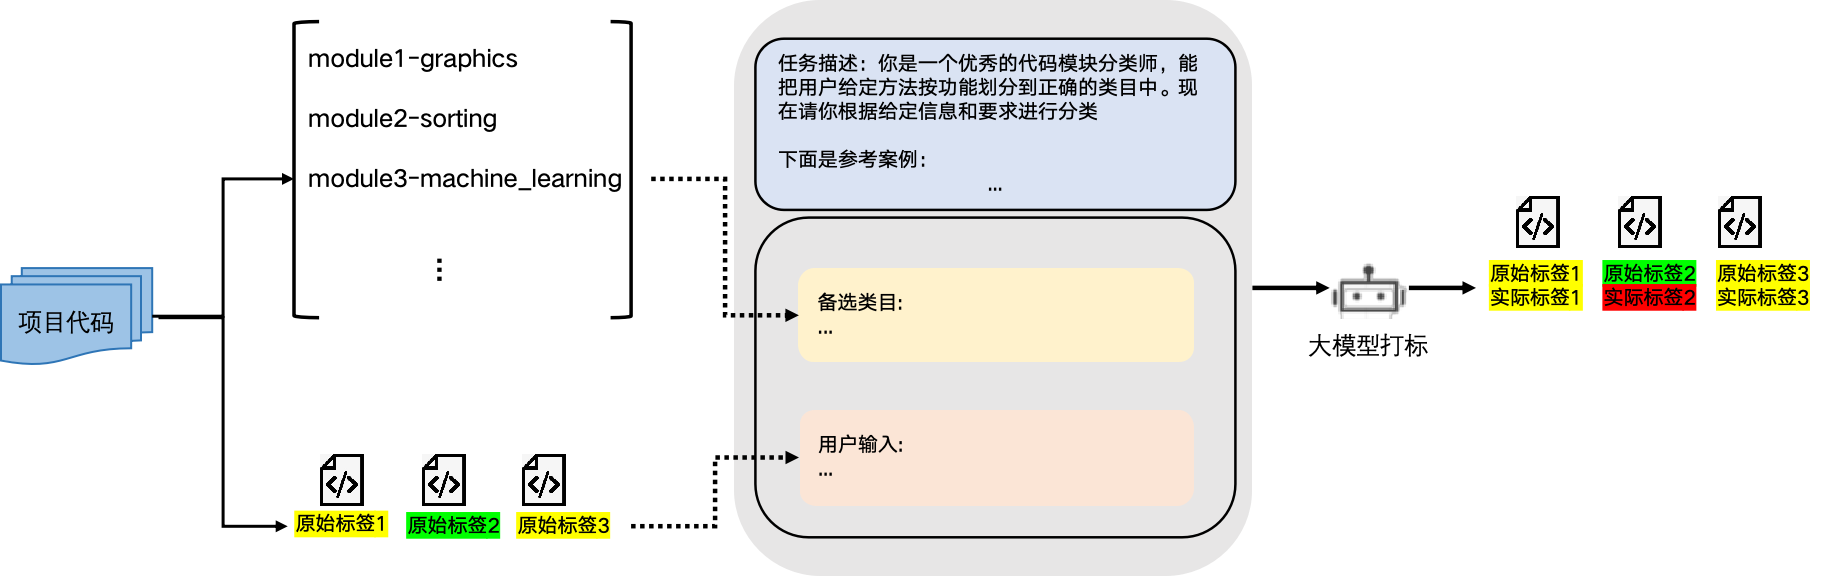
\includegraphics[width = 0.8\textwidth]{大模型预测.png}
    \caption{基于大语言模型的方法模块标签生成研究方案}
    \end{figure}

由于大语言模型的较强的理解和推理能力,并且经过验证,大模型具有良好的文本分类效果\cite{wan-etal-2023-gpt},而大模型对于代码的理解不差于对文本的理解,因此本文尝试使用大语言模型进行分类。研究方案如图4-1所示。


首先从项目代码中提取所有模块名,作为备选类目,提取方法的原始模块名并记录原始标签,将方法和备选类目组织成任务的描述,送给大模型进行打标,让其根据方法本身的功能,对方法进行分类打标,得到方法的实际标签。


\subsection{基于原始标签的方法分类}

大模型打标得到实际标签后,按项目的模块对方法进行分类。将模块名作为类别名,创建对应的一个个集合。遍历每一个方法,按方法的原始标签将方法放入对应的集合,完成分类。

\begin{figure}[h]
\centering
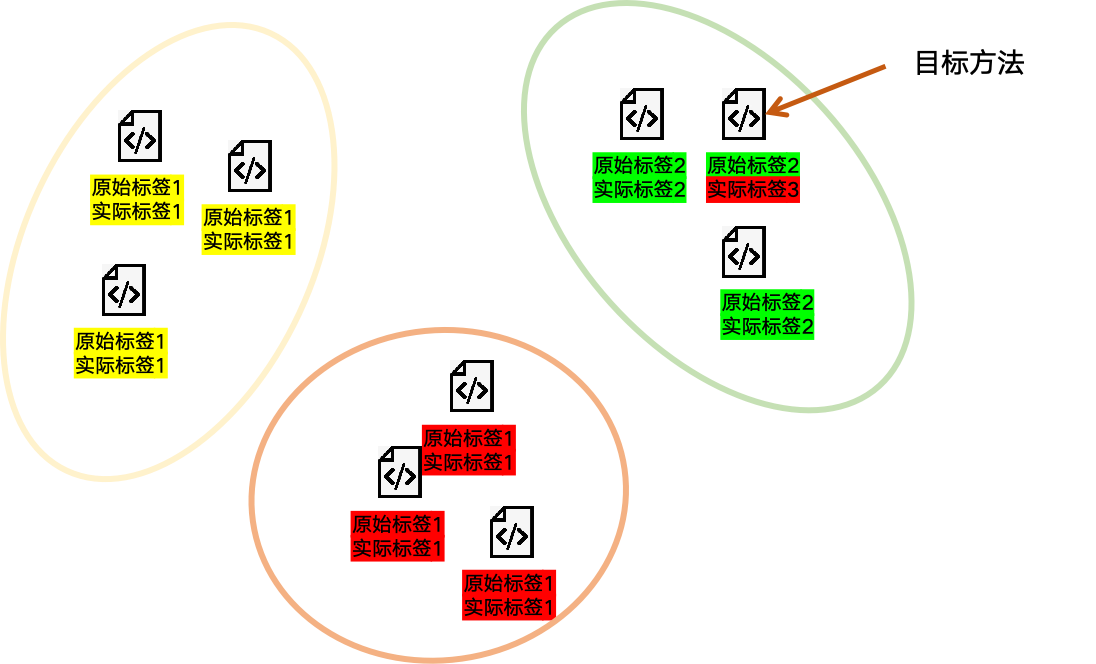
\includegraphics[width = 0.6\textwidth]{分类示例.png}
\caption{分类后实际标签与原始标签不符示例}
\end{figure}

分类结束后,我们会观察到这样的现象,每一个模块对应的方法列表中,会有实际标签并不是该模块的方法,这说明该方法是在代码维护过程中,被退化过程所影响的方法,用户应进一步观察该方法是否应在拆分到实际模块中。


\section{代码审查图}

\subsection{代码审查图构建}

代码审查图主要由两个核心元素构成,即节点和边。其中,节点代表软件项目中的方法或全局变量,边则表示节点之间的各种关系,如耦合关系、变更影响关系以及依赖调用关系。这些元素的结合能够帮助开发者从全局视角理解和评估项目的结构和质量,尤其是在进行代码审查和变更分析时。

(1)节点属性

在代码审查图中,节点的作用是标识项目中的方法和全局变量。通过前文所述的方法摘要表和全局变量信息表,我们为每个方法和全局变量创建了对应的节点。每个节点都具有多个属性,这些属性能够提供有关节点所代表的方法或变量的关键信息,便于开发者对代码进行全面的审查和分析。

方法属性分为两个主要部分:,首先是方法的基本信息,如表4-1所示。

\begin{table}[htbp]
\caption{代码审查图节点属性-基本信息}
\vspace{0.5em}\centering\wuhao
\begin{tabular}{cccc}
\toprule
    属性 & 描述 \\
\midrule
方法名 & 方法名,由方法所在路径和方法名拼接而成,保证唯一  \\
方法参数 & 方法的参数列表,包括参数的名称和类型   \\
方法内调用方法 & 本方法内调用的其他方法名   \\
方法可作用域 & 表明方法是否全局可用   \\
方法所在模块 &  方法所在模块,目前表示为方法所在文件  \\
模型预测方法模块 & 模型预测的方法应在的模块   \\     
\bottomrule
\end{tabular}
\end{table}

这一部分包括方法的名称、所在模块、方法签名、访问修饰符等基本信息,这些信息有助于开发者快速识别和定位方法的功能和作用。例如,方法的名称可以反映其业务功能,所在模块和调用信息则有助于理解方法的上下文和调用约束。

其次是与代码质量相关的度量和信息,如表4-2所示。

\begin{table}[htbp]
    \caption{代码审查图节点属性-质量相关信息}
    \vspace{0.5em}\centering\wuhao
    \begin{tabular}{ccp{9cm}}
    \toprule
    属性类别 & 属性 & 描述 \\
    \midrule
    \multirow{2}{*}{扇入扇出信息}& 扇入 &  方法的扇入值以及扇入值在项目中的排名比例 \\       
                                & 扇出 &  方法的扇出值以及扇出值在项目中的排名比例 \\   \cline{2-3}
    \multirow{2}{*}{内聚度信息}& LCOM1 &  所在模块的LCOM1值以及相应建议 \\       
                                & LCOM2 &  所在模块的LCOM2值以及相应建议 \\    
                                & LCOM3 &  所在模块的LCOM3值以及相应建议 \\    
                                & LCOM4 &  所在模块的LCOM4值以及相应建议 \\    
                                & TCC &  所在模块的TCC值以及相应建议 \\    
                                & LCC &  所在模块的LCC值以及相应建议 \\   \cline{2-3}             
    \multirow{2}{*}{耦合关系}& 数据耦合 &  与本方法存在数据耦合关系的方法 \\       
                                & 标记耦合 &  与本方法存在标记耦合关系的方法 \\   
                                & 外部耦合 &  与本方法存在外部耦合关系的方法 \\   
                                & 公共耦合 &  与本方法存在公共耦合关系的方法 \\   \cline{2-3}
    变更影响关系 & 变更影响关系 &  与本方法存在变更影响的方法,表明来源为代码克隆、变更历史、模型预测 \\    \cline{2-3}
    缺陷 & 静态代码缺陷 &  由cppcheck检测得到的本方法缺陷 \\      
    \bottomrule
    \end{tabular}
    \end{table}

这一部分基于前文方法提取和统计结果,涵盖了一些与代码质量直接相关的指标,如方法的扇入扇出、内聚度、耦合性等。这些度量和指标的结果将结合项目的具体统计数据或检测结果,向开发者提供有针对性的改进建议。例如,如果某个方法的扇出度位居项目中的前5\%,则可能表明该方法在项目中的依赖关系过于复杂,可能导致高耦合性,进而影响系统的灵活性和可维护性。类似地,如果检测出某方法存在不良耦合,则可能需要开发者重新设计该方法与其他模块的接口,以减少不必要的依赖。



对于全局变量的属性则主要包含表4-3中的信息。主要是对全局变量基本信息的展示,方便开发者快速了解该变量的作用域、使用情况以及与其他代码部分的关联性。通过这些信息,开发者能够更好地理解变量在整个项目中的作用及其潜在的质量风险。

\begin{table}[htbp]
\caption{代码审查图节点属性-全局变量信息}
\vspace{0.5em}\centering\wuhao
\begin{tabular}{cccc}
\toprule
    属性 & 描述 \\
\midrule
变量名 & 全局变量名,由所在路径和变量名拼接而成,保证唯一  \\
变量类型 & 变量类型   \\
被使用方法 & 使用了本全局变量的方法名   \\
变量可使用域 & 表明变量是否全局可用   \\
方法所在模块 &  变量所在模块,目前表示为所在文件  \\  
\bottomrule
\end{tabular}
\end{table}


(2)边的设计

在代码审查图中,边表示节点与节点之间的关系,这些关系揭示了软件系统中各个方法与全局变量之间的相互依赖和影响。根据其性质,边的类型主要分为三类,具体分类如表4-4所示:静态依赖关系、耦合关系和变更影响关系。

其中静态依赖关系分为方法之间的调用关系和方法与全局变量的引用,耦合关系如表4-2中所示共4类,变更影响关系则根据检测方法的不同,设定为3个不同的来源。需要注意的是,由于依赖闭包方法本身是基于依赖图生成的,因此在代码审查图中,这类关系不再单独指出。

每种关系反映了不同层次的代码相互作用,帮助开发者全面理解系统的结构和潜在的质量风险。

\begin{table}[htbp]
\caption{代码审查图边分类}
\vspace{0.5em}\centering\wuhao
\begin{tabular}{cccc}
\toprule
属性 & 描述 \\
\midrule
静态依赖关系 & 含方法之间调用、方法引用全局变量两种  \\
耦合关系 & 含数据耦合,标记耦合,外部耦合,公共耦合四种   \\
变更影响关系 & 含代码克隆、变更历史、模型预测三种  \\
\bottomrule
\end{tabular}
\end{table}



\subsection{代码审查图可视化}

本节从代码审查图的可视化方案和交互方案两个方面展开介绍。

1.可视化方案 

代码审查图的可视化方案基于开源项目 G6。G6 是一个强大的图形可视化引擎,提供了绘制、布局、分析、交互、动画等全方位的图形可视化基础功能,具有简单易用且完备的特性。G6 具有两个显著优势。

(1)数据与可视化图形分离:在使用 G6 时,用户只需将图的数据组织为 JSON 格式,如图4-3所示,包括节点信息和边信息,直接传递给 G6 即可自动生成对应的力导向图。这种数据与图形的分离不仅简化了开发流程,还提高了数据的灵活性和可操作性,便于进行后续的数据更新和图形重绘。

\begin{figure}[h]
\centering
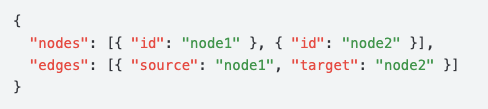
\includegraphics[width = 0.6\textwidth]{G6图数据示例.jpg}
\caption{G6图数据示例}
\end{figure}

(2)高度的定制能力:G6 提供了丰富的图形展示配置选项,用户可以根据需求自由选择不同的样式和布局方式。如果 G6 内置的元素不满足特定需求,它还支持用户自定义节点、边及其他元素,使得图形展示更加贴合实际应用场景。

本文使用G6内置节点和边实现代码审查图的可视化。G6的节点构成共包含6部分,其中label表示文本标签,通常用于展示节点的名称或描述,本文中将节点属性赋值给label,便于用户查看属性相关信息。G6的边的构成共包含4部分,label具有同样的功能,将边的类别用于label。让 G6 加载此数据源进行展示,就实现了同时也实现了计算逻辑与图形可视化的有效分离。


2.交互方案

对于软件项目这样的分析对象,方法和全局变量的数量常达到千级别,这样的级别对于一个图来讲,很难在图中展示完所有的信息,因此需要用户交互,来展示更详细的信息。表4-5展示了目前代码审查图的交互和对应的逻辑设计。

\clearpage




\begin{table}[htbp]
\caption{代码审查图交互和逻辑设计}
\vspace{0.5em}\centering\wuhao
\begin{tabular}{cccc}
\toprule
交互方式 & 业务逻辑 \\
\midrule
视角缩放 & 操作鼠标滚轮对图进行缩放  \\
视角移动 & 鼠标拖拽移动整个代码审查图   \\
聚焦节点 & 光标悬停在节点上显示节点的方法名/变量名  \\
移动节点 & 鼠标长按节点拖拽可移动节点 \\
查看节点属性 & 鼠标点击节点展开节点属性  \\
聚焦关系 & 光标悬停在边上显示边的类型  \\
查看关系信息 & 鼠标点击节点展开节点属性  \\
节点筛选 & 通过点击筛选节点按钮,确认是否筛选掉孤立节点 \\
\bottomrule
\end{tabular}
\end{table}



\subsection{代码审查报告生成}

在软件开发和代码审查的过程中,开发者通常可以借助代码审查图聚焦于代码的上下文,帮助发现局部代码的问题。然而,当软件开发完成,开发者希望从全局角度对软件项目的整体质量进行衡量时,仅依靠代码审查图可能会存在质量信息过于分散、不易聚焦的问题。因此,本研究进一步提出通过生成文档化的代码审查报告,为开发者提供统一的代码质量概览,帮助其全面掌握项目的质量状况。

代码审查报告的核心目标是揭示软件项目中存在的关键质量问题,并以本文提取的代码质量属性为主线,系统性地向用户报告代码中的潜在问题。具体来说,报告主要涵盖以下几个方面的内容:

\begin{itemize}
    \item 内聚度信息:报告中将重点标记内聚度最差的 5\% 模块,并提供相应的统计信息。这些模块通常在逻辑结构上松散、职责分散,可能是代码设计需要改进的关键部分。开发者可通过这些信息快速识别项目中存在高维护风险的模块。
    
    \item 不良的耦合信息:包括同模块内的公共耦合、不同模块的公共耦合以及外部耦合。这些耦合关系可能导致模块之间的高依赖性和低灵活性,影响系统可维护性。
    
    \item 复杂度信息:报告将筛选出扇入扇出指标最差的 5\% 模块,提供详细数据说明。这些模块往往由于过多的依赖关系或调用关系而难以维护,是优化的重点对象。
    
    \item 代码缺陷与规范信息:cppcheck 检测出的代码缺陷和不符合规范的代码信息,并给出相应的建议。
    
    \item 不良变更影响:通过分析代码中的变更影响关系,报告将重点指出项目中存在变更影响关系数量最多的前 5\% 方法。这些方法通常具有较高的变更复杂度,是项目维护中的风险点。
    
    \item 基于大模型的模块预测结果:报告列出那些标签不属于原始模块的方法名称。此类方法可能存在职责划分不当或模块归属不合理的情况,报告将此信息提供给用户,供其判断是否需要重新划分模块归属,从而优化模块结构。
\end{itemize}

为了帮助用户在代码开发过程中防止变更不完全,报告还将列出项目中所有的代码变更影响关系。用户可以参考这些信息,在变更时全面评估影响范围,降低遗漏风险。

通过对这些信息的整合与分析,生成的报告文档为用户提供了一份全面的代码质量概览,既可以帮助用户识别代码中的潜在问题,又能为系统的后续优化与维护提供指导性建议。

\section{实验结果与分析}

\subsection{实验环境与评价方法}

本章依旧使用第二章中的项目为示例项目。

(1)实验环境

实验环境如表4-6所示。

\begin{table}[htbp]
\caption{实验环境}
\vspace{0.5em}\centering\wuhao
\begin{tabular}{cccc}
\toprule
    环境 & 信息 \\
\midrule
操作系统 & macOS Ventura v13.5.2  \\
Intellij pycharm & 2021.1.1   \\
python & 3.7   \\
Java & 1.8   \\
G6 & g6.min.js 4.3.11  \\  
libclang & 15.0.7  \\ 
pycparser & 2.21  \\
\bottomrule
\end{tabular}
\end{table}

对于基于大语言模型的方法模块标签生成方法,本文使用了Doubao-lite-4k-240828、Doubao-lite-32k-240828、Spark Lite共三种大语言模型进行实验。

(2)评价方法



对于基于标签生成的模块分类方法,我们首先需要验证大模型进行方法模块分类的准确性,只有当分类准确时,才能信任其对于方法拆分的建议。虽然没有真实标签,但是项目中的大部分方法都应属于原始标签,因此本文首先计算预测的实际标签和原始标签相等的比例。如果比例较高,则说明大模型预测模块有一定准确性,则进一步实例分析实际标签和原始标签不同的案例,验证其可行性。

对于代码审查图生成方法,首先对示例项目生成代码审查图,验证可视化方案的需求,根据代码审查图分析前文中实验结果中的实例研究,以说明代码审查图相较文字的优越之处。

对于代码审查报告的生成,则是验证审查报告的格式是否符合设计方案。

\subsection{实验结果与实例分析}

1. 大语言模型模块分类实验结果

示例项目中,预测的实际标签和原始标签相等的比例如表4-7所示。


\begin{table}[htbp]
\caption{变更影响接受率实验结果}
\vspace{0.5em}\centering\wuhao
\begin{tabular}{cccc}
\toprule
项目名称 & Doubao-lite-4k-240828 & Doubao-lite-32k-240828 & Spark Lite \\
\midrule
antiword & 66.2 & 73.4 & 43.1 \\
librdkafka & 42.1 & 45.3 & 33.7 \\
TheAlgorithms & \textbf{84.2} & 87.2 & \textbf{63.2} \\
libbpf & 83.7 & \textbf{96.2} & 53.1 \\
FFmpegKit & 40.6 & 57.7 & 31.7 \\
jemalloc & 60.6 & 60.3 & 39.8 \\
\bottomrule
\end{tabular}
\end{table}

总的来讲,实际标签和原始标签相等的比例并不低,有的项目甚至可达90以上,这说明大部分的方法实际标签等于原始标签的假设是有一定可信度的。单项目内横向对比,可以发现Doubao-lite-32k的比例大于Doubao-lite-4k,两个模型的比例都高于SparkLite,这可能是由于模型的性能问题。

为了使模块拆分的建议更具可信性,选择准确率较高的TheAlgorithms项目进一步分析。首先经过分析可以发现,该项目的文件命名和方法命名非常准确,见名知义,因此模型预测都较为准确,由此可以看出,模块命名是否规范,对模块预测具有较强的影响。其次对Doubao-lite-32k-240828模型预测的实际和预测并不相等的例子进行抽样分析,共167个方法,抽取其中50个方法进行分析,用户共接受了7个方法,接受率14.0\%,并不高。但是通过用户接受的例子也能发现,该方法有一定的实际意义。

\begin{table}[htbp]
\caption{TheAlgorithms项目中预测与实际不符的实例统计}
\vspace{0.5em}\centering\wuhao
\begin{tabular}{cccc}
\toprule
预测与实际不符方法总数 & 抽样 & 用户接受 & 所占比例 \\
\midrule
167 & 50 & 7 & 14.0\% \\
\bottomrule
\end{tabular}
\end{table}


2. 代码审查图

(1)代码审查图概览

图 4-4 展示了 Antiword 项目和 TheAlgorithms 项目的代码审查图,直观地反映了两者的结构特征和模块化差异。图中,圆形节点表示方法,方形节点表示全局变量,不同颜色的边则代表了代码元素之间的不同关系:蓝色边表示依赖关系,绿色边表示耦合关系,红色边表示代码变更影响关系。上方的图是未区分模块的全局视图,所有的节点和边混杂在一起,仅从整体上体现了项目的结构复杂度。而下方的图对模块进行了区分,采用颜色区分不同模块,将属于同一模块的节点用相同颜色进行标注,从而进一步突出模块之间的边界和逻辑关系。

\begin{figure}[!h]
    \setlength{\subfigcapskip}{-1bp}
    \centering
    \begin{minipage}{\textwidth}
    \centering
    \subfigure[antiword-未划分模块]{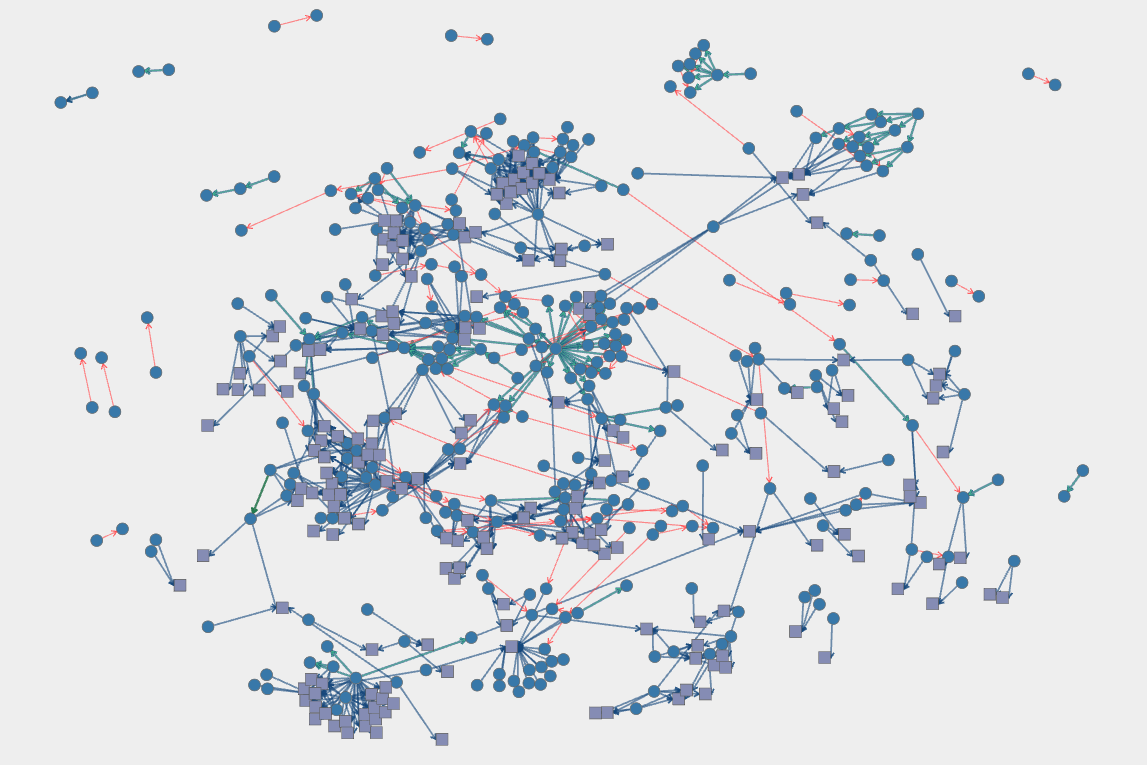
\includegraphics[width=0.4\textwidth]{antiword审查图未上色.jpg}} % 保留中文标题
    \hspace{2em}
    \subfigure[TheAlgorithms-未划分模块]{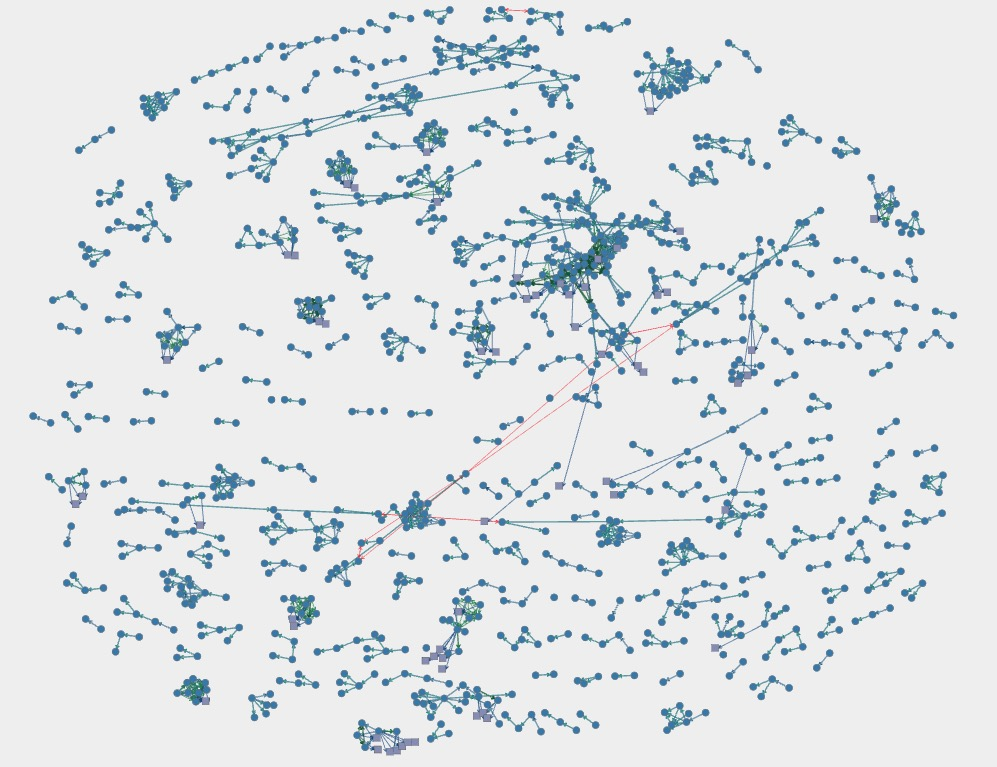
\includegraphics[width=0.4\textwidth]{aigri代码审查图-未上色.jpg}} % 保留中文标题
    \end{minipage}
    \centering
    \begin{minipage}{\textwidth}
    \centering
    \subfigure[antiword-划分模块]{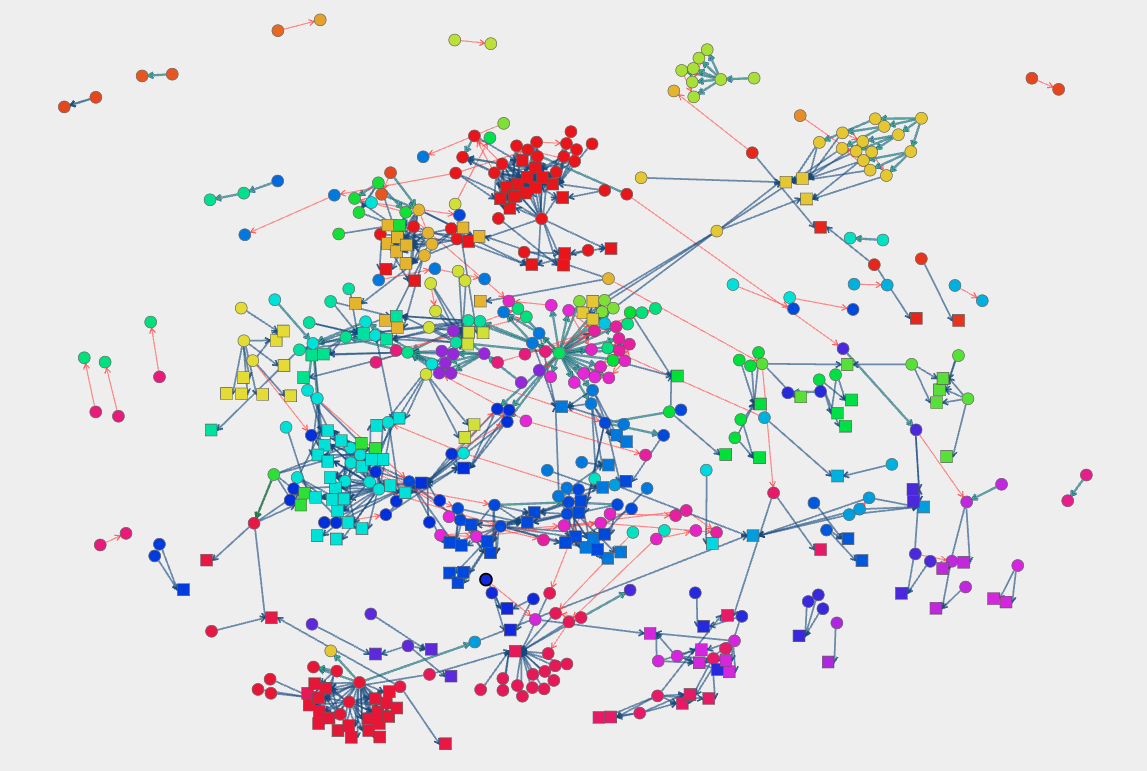
\includegraphics[width=0.4\textwidth]{antiword代码审查图.jpg}} % 保留中文标题
    \hspace{2em}
    \subfigure[TheAlgorithms-划分模块]{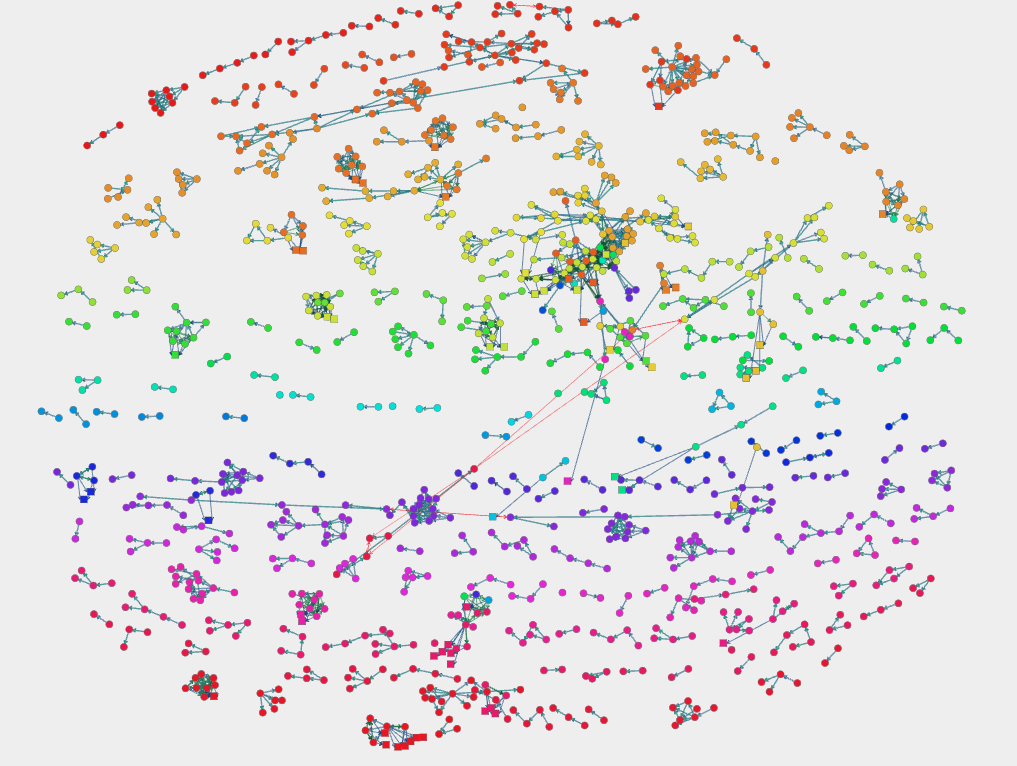
\includegraphics[width=0.4\textwidth]{aigri代码审查图.jpg}} % 保留中文标题
    \end{minipage}
    \vspace{0.2em}
    \caption{代码审查图} % 只保留中文标题
\end{figure}


从图中可以明显看出两个项目在结构特征上的显著差异。Antiword 项目整体模块之间高度协作,共同实现一个完整的功能,因此模块之间的联系较为紧密,表现出较强的耦合性。从可视化图上观察,按模块划分后,可以清晰地看到具有相同功能的模块形成了较为紧密的聚集。同一颜色的节点集中分布,进一步体现了模块的内聚性较高以及逻辑结构的清晰性。

相比之下,TheAlgorithms 项目由于其作为算法库的特性,方法之间的耦合性较低,各模块间的联系相对较弱。从图上来看,不同模块呈现出较为分散的分布,模块内部的聚集程度也较低。整体结构表现为由若干独立模块组成,松散而分离,符合库函数式项目的典型特征。

\begin{figure}[h]
\centering
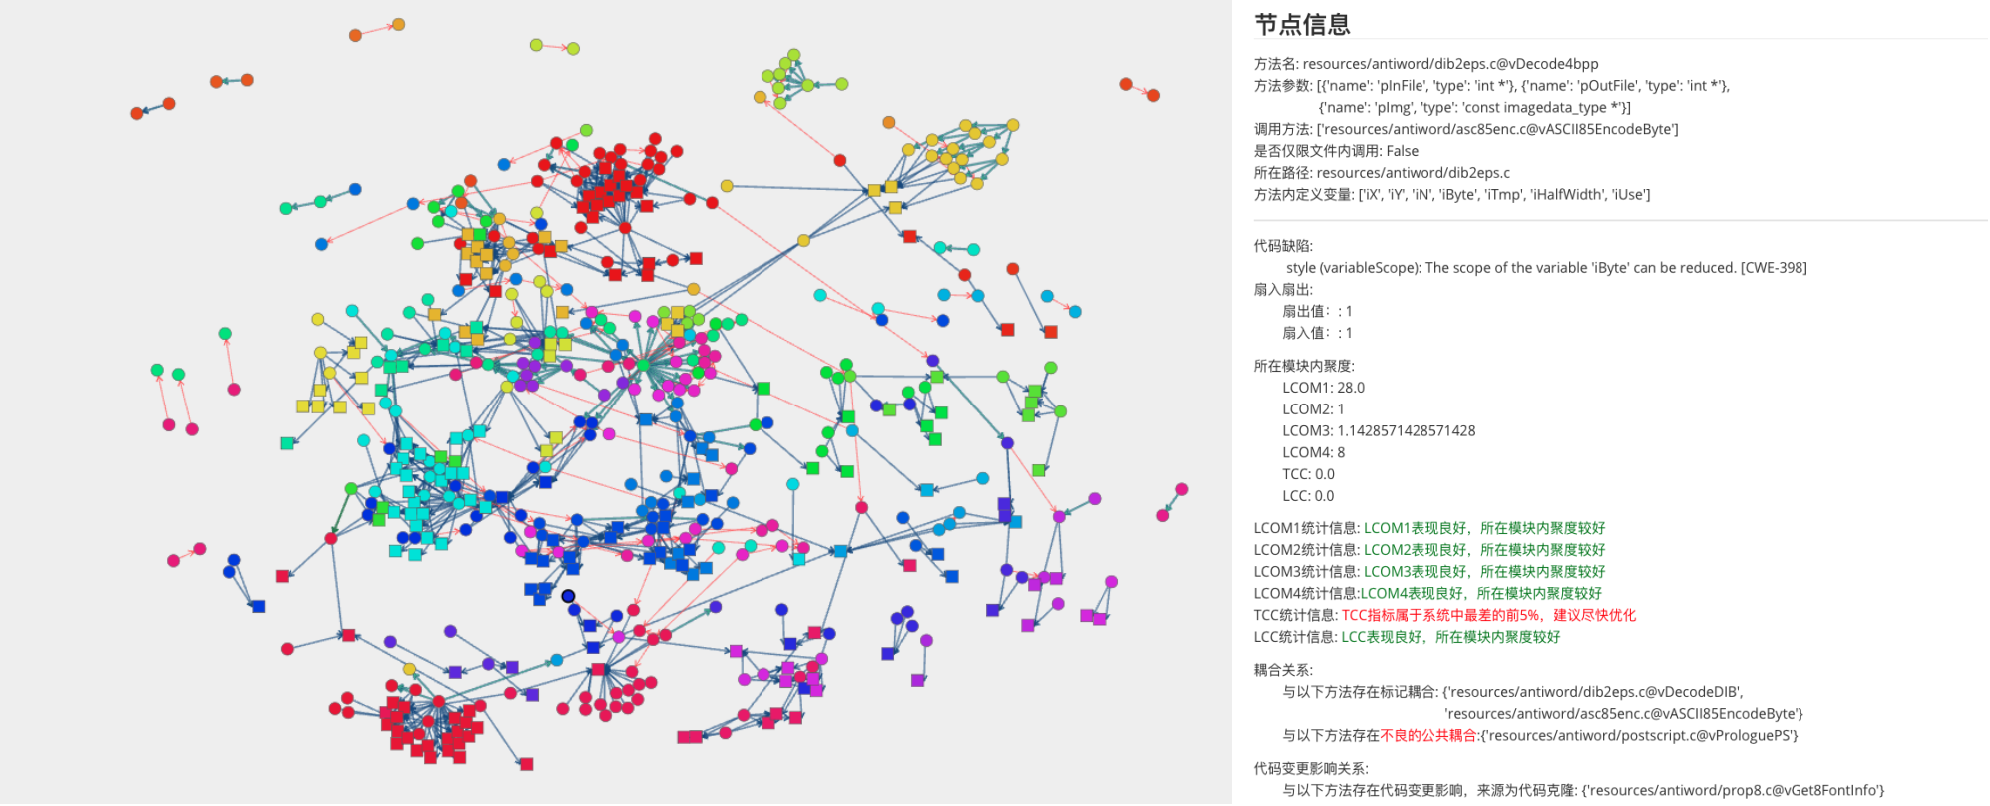
\includegraphics[width = 1\textwidth]{点击节点.png}
\caption{点击节点展开节点信息}
\end{figure}

此外,用户可以通过点击图中的某个节点来查看该节点的详细信息,包括方法或全局变量的具体描述。这一功能能够帮助用户快速定位关键信息,深入了解特定方法或变量的功能和用途,从而更高效地进行代码审查和理解。



(2)子图展示

代码审查图蕴含了丰富且有价值的信息,通过聚焦于代码审查图中的子图,开发者和审查者可以快速直观地理解代码结构之间的关系。子图清晰地展示了代码结构之间的依赖、耦合以及变更影响关系,使得复杂的代码逻辑更加可视化。

以 antiword 项目中的子图为例,本文聚焦于 vDecodeDIB 方法的代码开发和审查场景。若按照传统方法对该方法进行开发或分析,仅通过人工阅读代码,开发者需要深入解析与其相关的依赖关系和变更影响关系,这可能涉及 300 多行代码的逻辑才能全面掌握方法的上下文。然而,通过代码审查图,开发者只需关注 8 个节点和 9 条边,即可快速获取关键信息。这种直观的可视化显著降低了代码理解的复杂度和成本。

\begin{figure}[h]
\centering
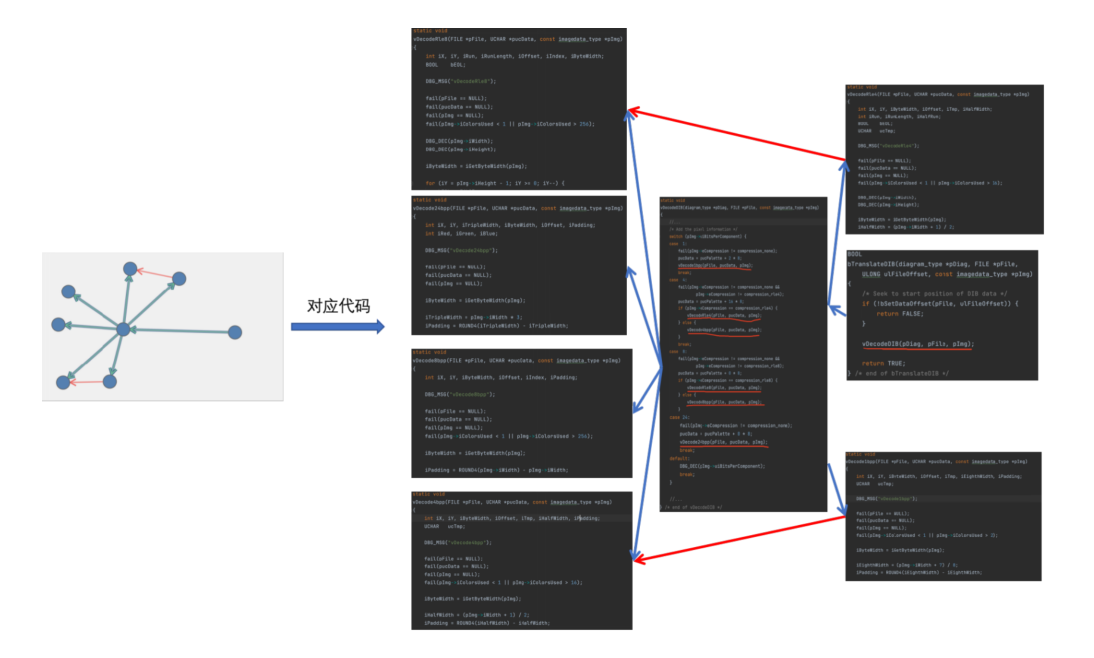
\includegraphics[width = 1\textwidth]{代码审查图子图.jpg}
\caption{vDecodeDIB方法上下文}
\end{figure}

尤其值得注意的是,变更影响关系中包含了两个基于克隆代码的关系。这类关系通常隐匿于代码中,开发者仅靠手动查看代码很难准确发现并记录。代码审查图将这些隐藏的克隆关系显式标出,使开发者在代码修改时能够快速识别潜在的影响范围,从而避免遗漏变更的风险。

对开发者而言,代码审查图能够提供更加直观的视角,帮助其快速掌握代码之间的各种依赖关系和耦合情况。在代码开发过程中,审查图不仅有助于理清模块间的关系,还能有效避免变更不完全的问题。而对于代码审查者,审查图能够快速展示代码的上下文结构,简化复杂逻辑的理解过程,同时高效地识别代码中的变更缺陷。

(3)代码质量属性体现

通过代码审查图,不仅可以直观展示代码的依赖关系和变更影响关系,还能有效地体现代码质量的特征,从而辅助用户理解代码质量较差或较好的具体原因。在第 2.6.2 节中详细解释了 misc.c 文件内聚度表现最差的原因,并统计了该文件内部方法和变量的相关信息。然而,仅依靠文字说明可能难以全面传达问题的全貌,而配合代码审查图,如图4-7所示,可以更加直观地展示该模块的结构问题。

\begin{figure}[h]
\centering
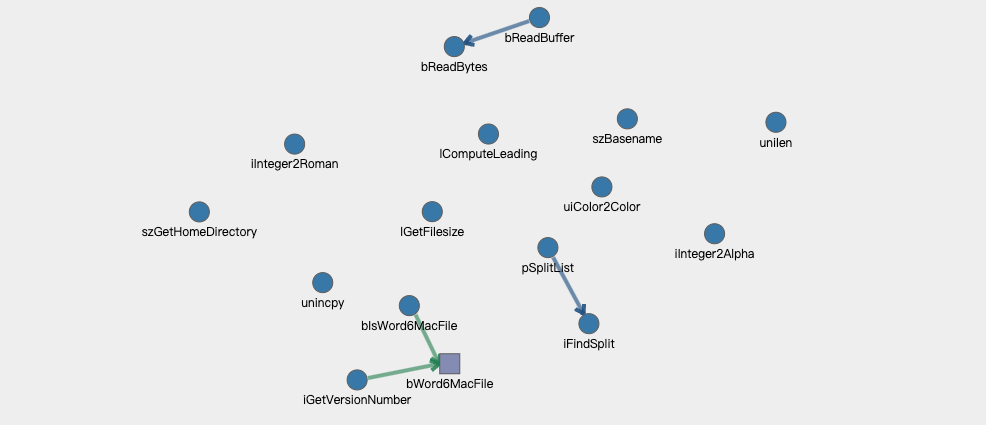
\includegraphics[width = 0.7\textwidth]{内聚度差例子.jpg}
\caption{misc.c 文件对应的代码审查图}
\end{figure}

从图中可以清晰地看出,misc.c 文件的结构非常松散,其内部存在大量孤立节点,缺乏足够的联系和协调关系。这些孤立节点既无法与其他节点形成有意义的逻辑关系,也难以体现出模块内部的高内聚性特征。这种松散的结构正是导致其内聚度表现最差的主要原因。

除此之外还有一些内聚度差和好的模块在代码审查图中可以清晰地展现,如图4-8所示。图中,左侧展示的是内聚度较差的模块,而右侧则展示了内聚度较好的模块。单纯从代码本身出发,往往难以直观地识别出导致内聚度差或较好的具体原因。然而,通过代码审查图,问题的根源得以清晰呈现。具体来说,左侧内聚度差的模块之所以表现为低内聚度,主要是因为存在过多的链式调用,这种设计使得模块之间的依赖关系过于松散,缺乏足够的内在联系。而右侧内聚度良好的模块,则表现出较强的模块化特征,模块内部功能紧密相关,依赖关系清晰且有序,从而促进了代码的高内聚性。通过这种可视化的方式,代码审查图不仅帮助开发者迅速识别出模块内聚度的优劣,还能够为后续的重构与优化提供建议,如左侧内聚度差的模块,可通过合并方法,减少方法数和调用量,达到提高内聚度的效果。

\begin{figure}[!h]
    \setlength{\subfigcapskip}{-1bp}
    \centering
    \begin{minipage}{\textwidth}
    \centering
    \subfigure[内聚度差——存在链式调用]{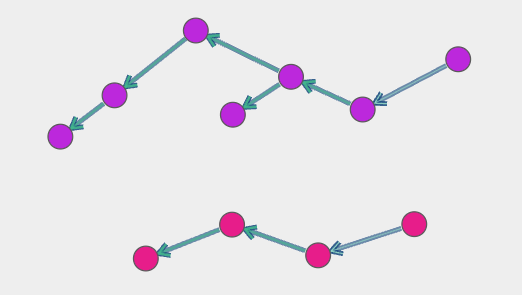
\includegraphics[width=0.4\textwidth]{存在链式调用.jpg}} % 保留中文标题
    \hspace{2em}
    \subfigure[内聚度良好——关联紧密]{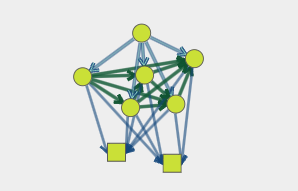
\includegraphics[width=0.4\textwidth]{内聚度好.jpg}} % 保留中文标题
    \end{minipage}
    \vspace{0.2em}
    \caption{内聚度良好和较差的例子} % 只保留中文标题
\end{figure}


在2.6.2节中对高扇出方法的讨论中,高扇出通常意味着方法存在过高的复杂性,这种特征在代码审查图中表现为具有大量的出边的中心化节点。如图4-9所示。图中的中心节点通过大量出边与其他模块或方法产生关联,这种结构不仅揭示了方法的复杂性,也反映了其可能导致的维护难度和潜在的设计缺陷。用户可以通过代码审查图迅速定位到具有高扇出的具体方法,深入了解其上下文信息,进而判断其是否存在不合理的复杂度。当发现高扇出的原因主要源于过多的依赖关系时,开发者可以及时采取相应的优化措施,如重构该方法、简化其职责或调整其与其他模块的关系,从而有效提升系统的可维护性和可扩展性。

\begin{figure}[h]
\centering
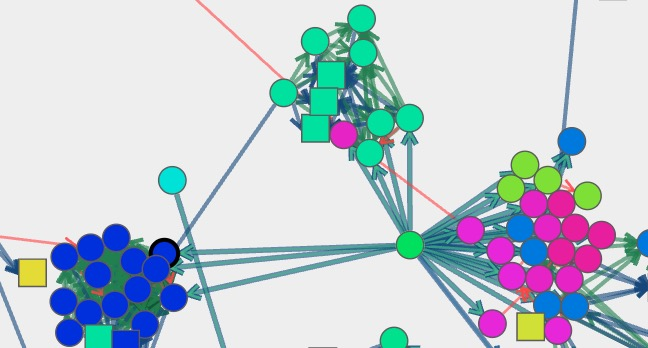
\includegraphics[width = 0.4\textwidth]{扇出度最高.jpg}
\caption{扇出度较高的节点}
\end{figure}

对于某些方法,其功能可能已经与当前所在模块的职责不再完全匹配,而与其他模块的结合更加紧密。这一问题在代码审查图中得以有效呈现。得益于力导向图的可视化特性,图中会显示出方法之间的依赖关系与耦合关系,紧密依赖的节点往往聚集在一起。由于同一模块内的节点通常会被赋予相同的颜色,若模块划分不合理,则会出现如图4-10所示的情况。在图中,聚集的节点颜色并不统一,某些节点(如图中的绿色和蓝色节点)与模块的主色调(橙色)不符。这表明,尽管这些方法本应属于其他模块,但它们与当前模块(即橙色模块)之间的耦合关系更为紧密。通过这种可视化,用户能够明确识别出不合理的模块划分,并采取相应的重构措施,例如将这些方法迁移至更合适的模块中,避免产生不良的耦合关系。这种调整不仅能够优化模块的功能划分,还能提高系统的可维护性与可扩展性,减少未来修改时的复杂度。


\begin{figure}[h]
\centering
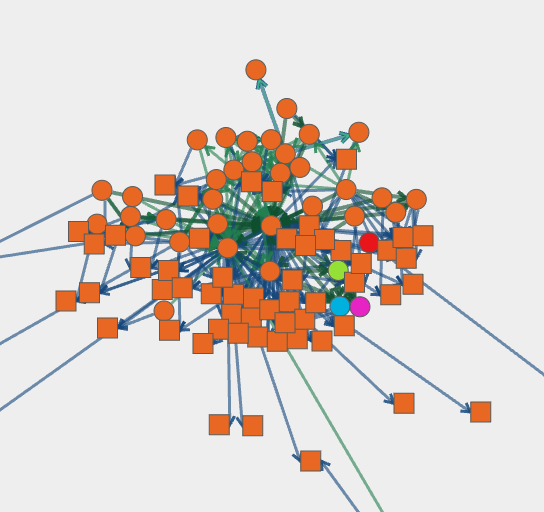
\includegraphics[width = 0.4\textwidth]{模块分错.jpg}
\caption{模块划分不合适的方法}
\end{figure}


在代码审查图中,我们也能看到一些方法之间的不良变更影响关系。除了直接反映变更影响较多的方法外,代码审查图还能够揭示出由于变更影响分析所导致的模块间不良变更传播问题。如图4-11。该子图涉及三个模块,每个模块的内聚度均较为良好,然而每个模块内都有一个方法与其他两个模块之间存在变更影响关系。这导致当这几个方法变动时,可能影响到不属于同一模块的代码也要跟着改变。更为严重的是,随着变更的涟漪效应,这些变更会进一步扩散,影响到更多模块,造成不必要的连锁反应。这种现象揭示了该系统架构存在潜在的问题——尽管各模块内部结构较为合理,但模块之间的依赖关系过于复杂且紧密,增加了维护和变更时的复杂度和风险。为解决这一问题,优化的建议是尽量减少或消除这种不良的变更影响关系。具体而言,可以通过提取和复用模块间的共同代码逻辑,消除不必要的代码克隆,进而降低跨模块变更传播的可能性。


\begin{figure}[h]
\centering
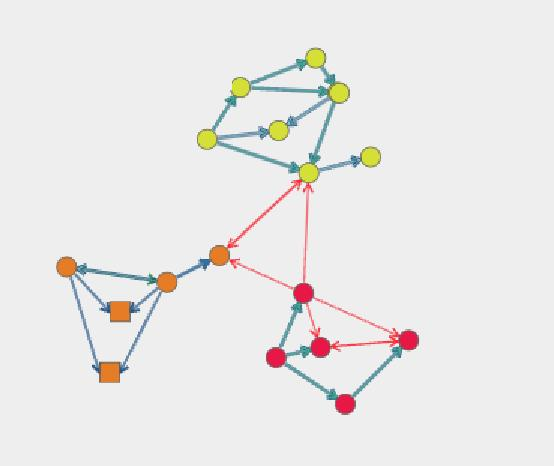
\includegraphics[width = 0.4\textwidth]{变更影响关系审查图.jpg}
\caption{不良的变更影响关系}
\end{figure}


总而言之,通过代码审查图,不仅能够帮助开发者快速定位模块质量问题,还能直观地理解问题的根源,为后续的优化和改进提供清晰的建议。这种结合文字与图形的分析方式,显著提升了代码质量评估的直观性和说服力。

3. 代码质量评估报告

下图展示了一个实际的代码评估报告示例。由于报告内容较长,这里仅展示了其中的一部分信息。通过代码评估报告,用户能够以结构化的清单形式全面了解软件项目中存在的各类质量问题及其具体位置。这些报告不仅清晰地列出了每个问题的详细描述,还提供了针对性优化或重构的建议。通过这种方式,开发团队可以快速识别代码中的潜在缺陷或性能瓶颈,并根据报告中提供的指导意见,采取有效的措施进行改进。报告的可视化和条目化呈现,帮助用户直观地理解各项问题的优先级和重要性,从而优化项目的维护流程,并提高软件系统的整体质量。

\clearpage

\begin{figure}[h]
\centering
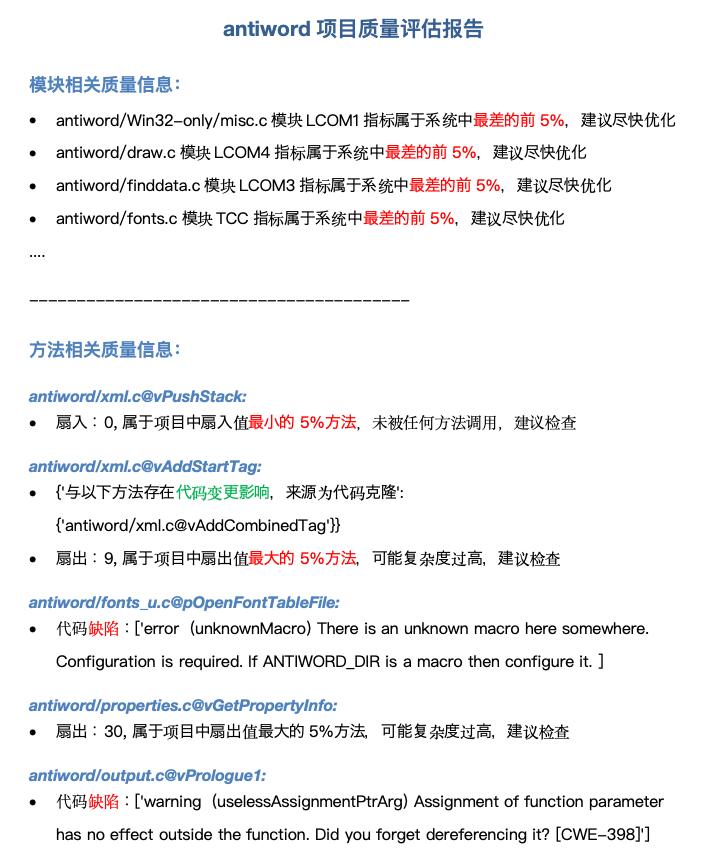
\includegraphics[width = 1.0\textwidth]{质量评估报告.jpg}
\caption{antiword项目代码质量评估报告节选}
\end{figure}


\section{代码审查图的实际应用}

在实际应用中,代码审查图可以有以下三种用法。

\paragraph{辅助开发者的代码维护} 当用户对软件代码进行开发时,可将复杂庞大的项目先通过系统进行分析,得到代码审查图。

\begin{figure}[h]
\centering
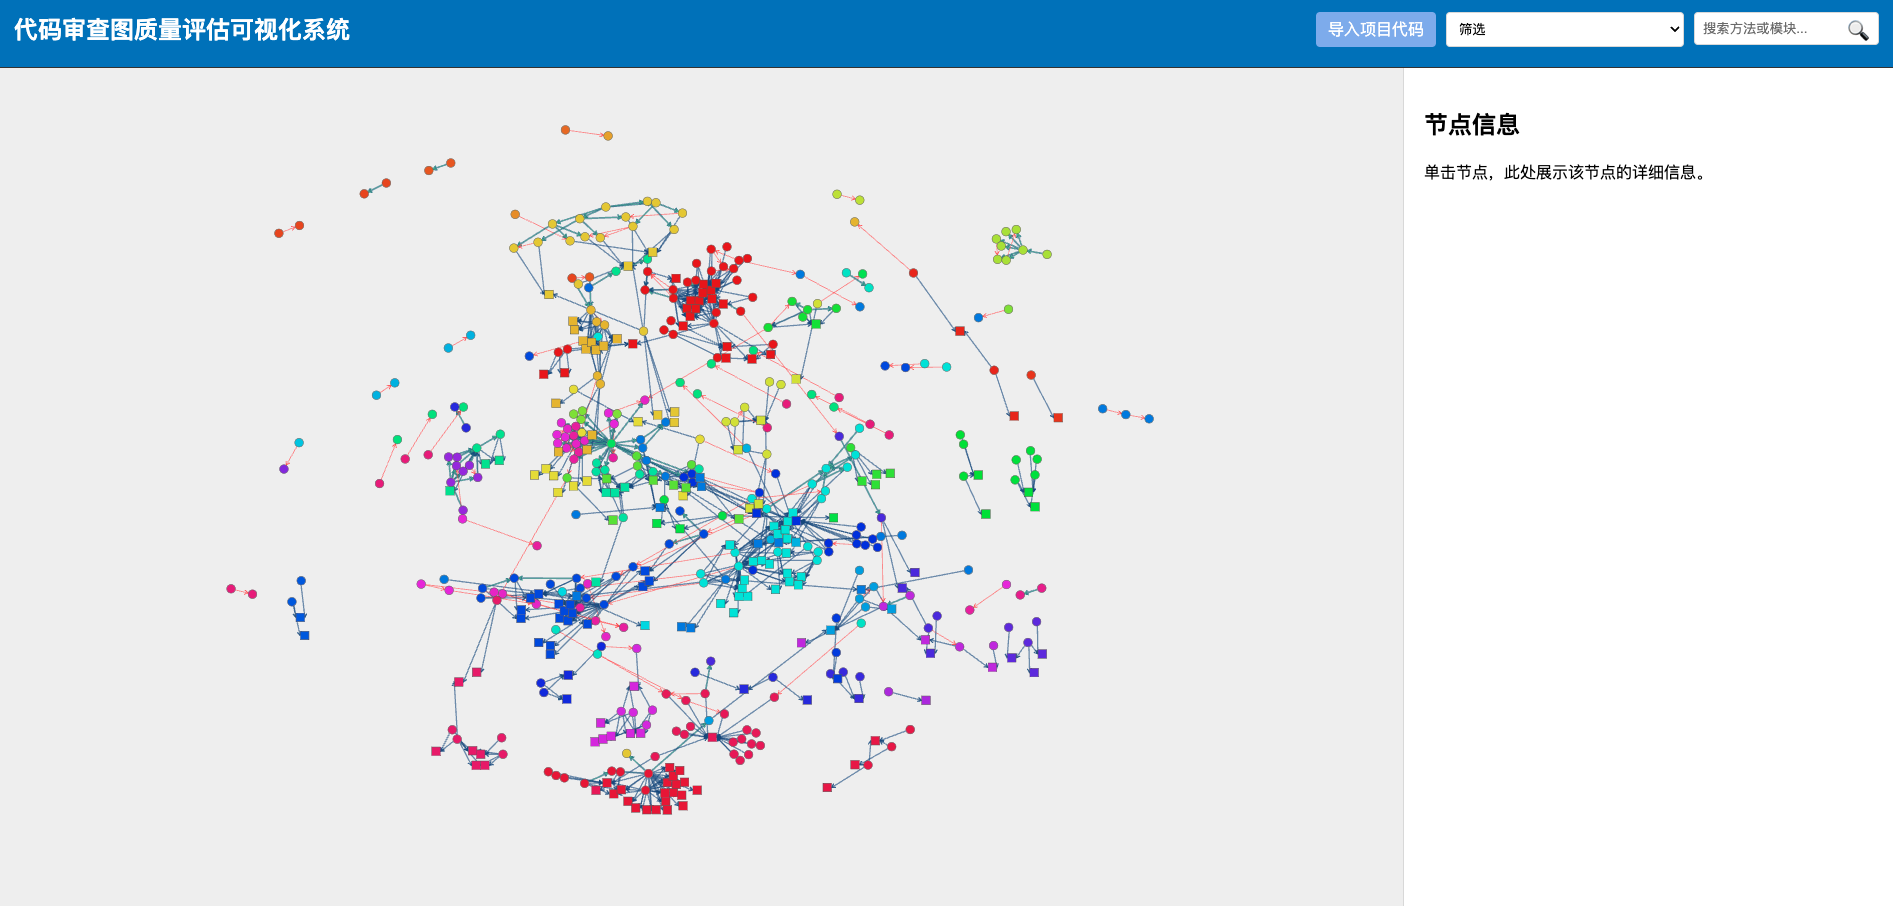
\includegraphics[width = 1.0\textwidth]{应用展示审查图.jpg}
\caption{导入项目生成代码审查图}
\end{figure}

对于开发任务所在的代码上下文,通过搜索方法名找到其在代码审查图中的位置,点击节点查看方法详细信息和质量情况,用户可根据相应的建议进行修改,优化代码质量。

\begin{figure}[h]
\centering
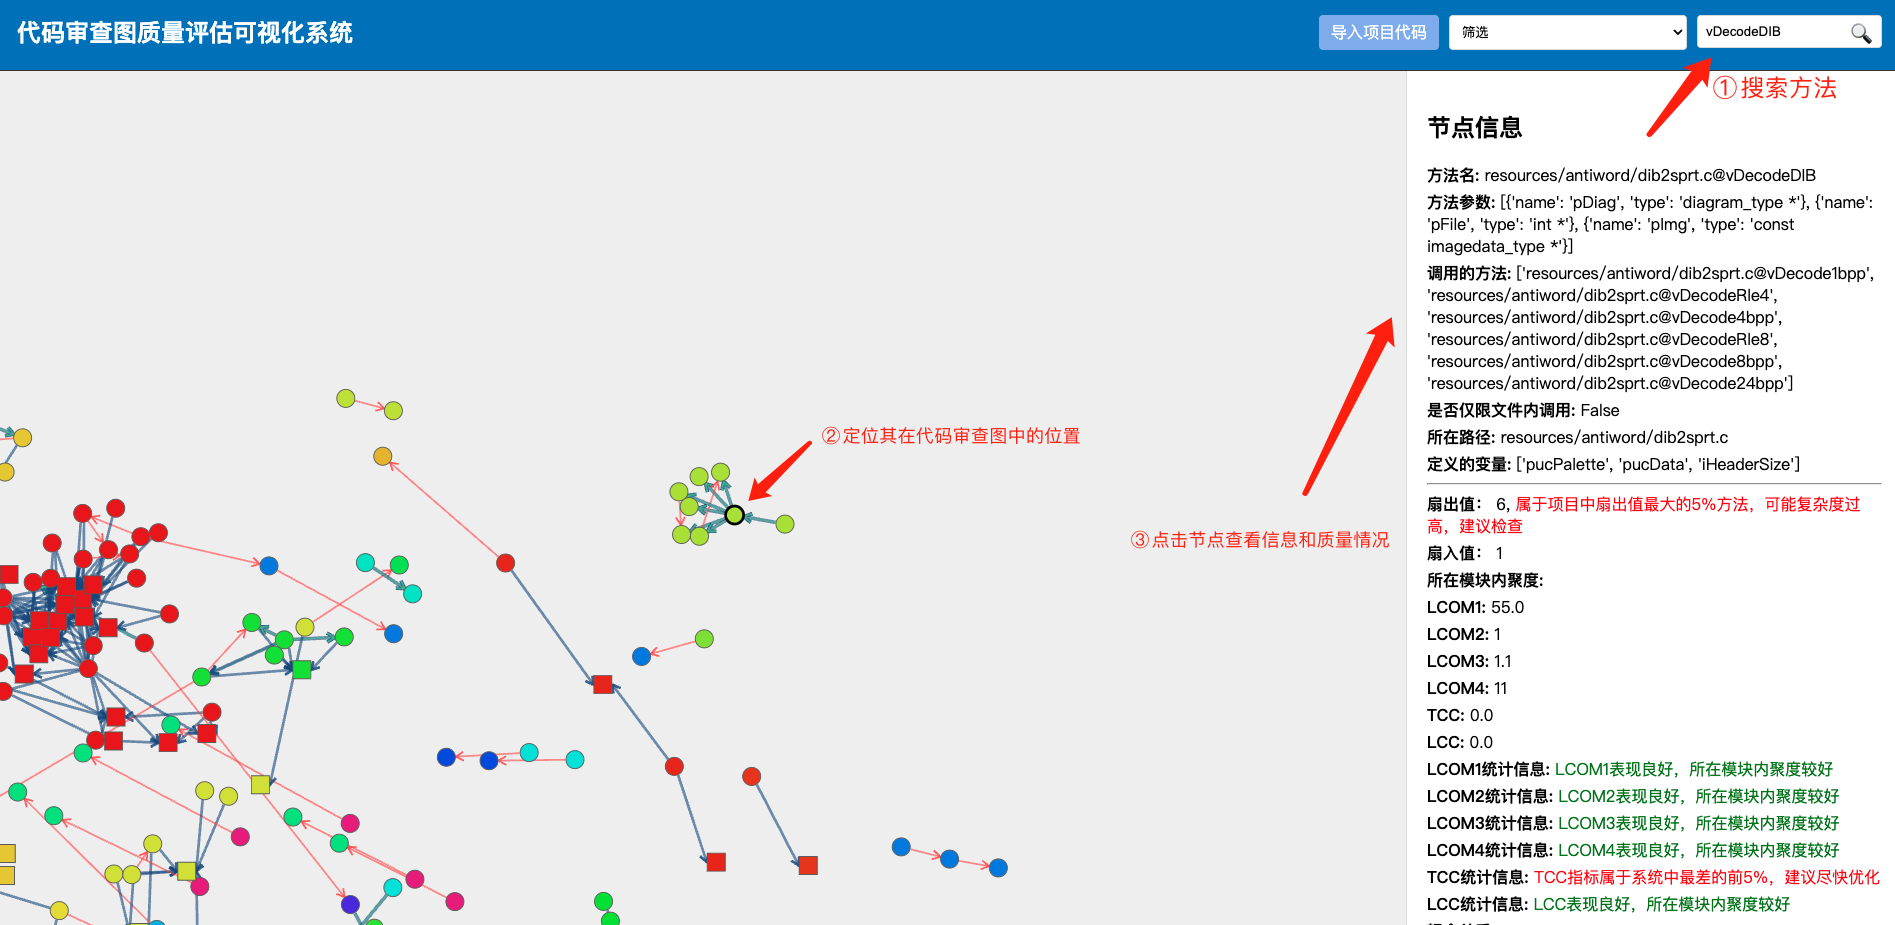
\includegraphics[width = 1.0\textwidth]{应用查看节点信息.jpg}
\caption{定位开发任务涉及的方法,查看质量信息}
\end{figure}

根据代码审查图的边,则可以了解当前代码与其他部分的依赖关系、耦合关系和变更影响关系。尤其是变更影响关系,可以帮助用户在进行变更时,提示其依赖型和逻辑型影响的范围,并根据给出的建议,帮助用户安全变更,解决了用户面对复杂软件难以理解、不敢变更、容易变更不完全的痛点。

\begin{figure}[h]
\centering
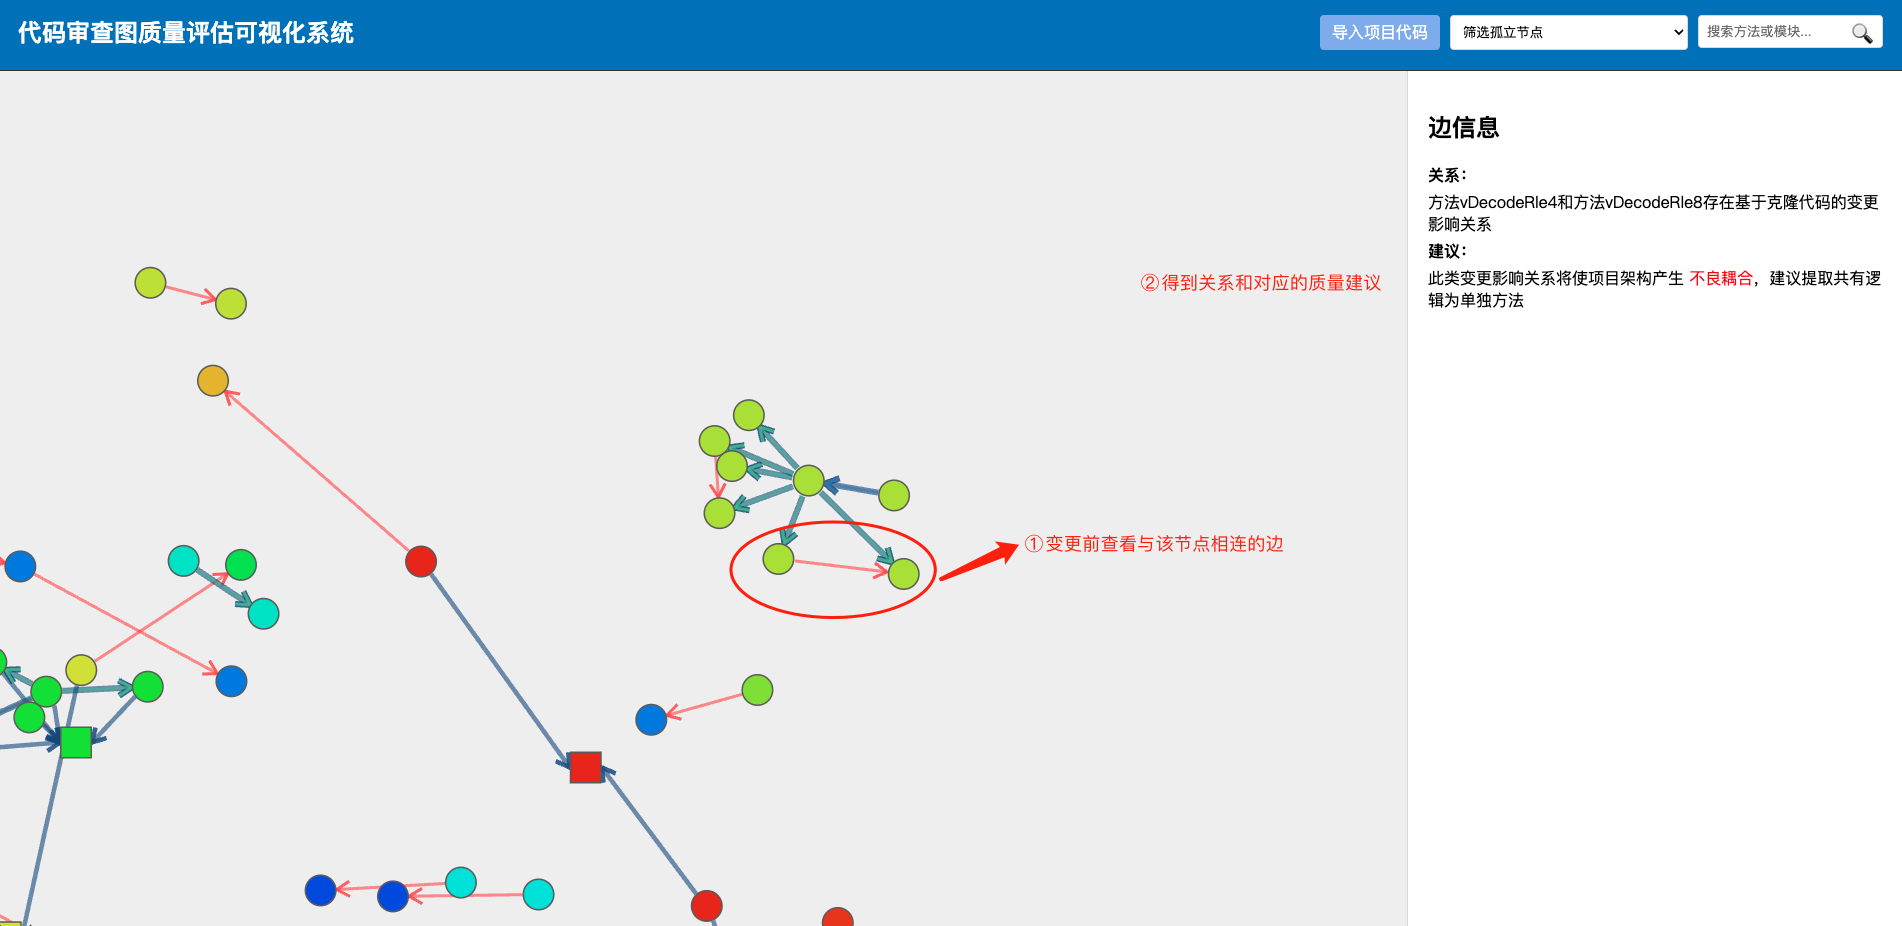
\includegraphics[width = 1.0\textwidth]{应用边信息.jpg}
\caption{查看方法对应边,按建议安全变更}
\end{figure}

\paragraph{作为审查工具帮助审查者进行审查} 当面对审查任务时,审查者可通过搜索代码审查图定位到当前提交所涉及的节点,通过图中的关系迅速了解代码上下文间的调用以及变更影响关系,通过系统的提示,对开发者的变更进行审查,检查其功能逻辑上是否安全变更,检查其变更操作给软件带来的质量影响是恶化还是优化,从而给出对应的审查结果。

\paragraph{作为质量评估工具对软件代码进行整体的评估} 用户可根据代码审查图,观察软件模块划分,也可导出代码质量评估报告,以清单的方式了解项目代码的质量情况。



\section{本章小结}

本章介绍了基于标签生成的方法模块分类,该方法通过大语言模型生成方法的实际标签进行分类,表明模块划分不正确的方法,通过实验证明,该方法具有一定的参考意义。其次介绍了代码审查图,将软件分析结果以图的形式展示给用户,方便用户从宏观的角度了解项目结构,最后介绍了代码质量报告的生成,通过清单式的质量信息报告,方便用户查询和优化。





% Local Variables:
% TeX-master: "../main"
% TeX-engine: xetex
% End:
